%-------------------------------------------------------------------------------
%                            BAB IV
%               		HASIL DAN PEMBAHASAN
%-------------------------------------------------------------------------------
\fancyhf{}
\fancyfoot[C]{\thepage}
\chapter{HASIL DAN PEMBAHASAN}
\section{ANALISIS KEBUTUHAN}

Hasil dari analisis kebutuhan yang telah dilakukan adalah mendapatkan kelompok pengguna yang akan terlibat dalam penelitian dan \textit{use case diagram} untuk masing-masing pengguna. Berikut hasil analisis kebutuhan dari sistem yang dibangun.
\subsection{Kelompok Pengguna}
Kelompok pengguna dari aplikasi ini telah dapat diidentifikasikan pada tahap analisis kebutuhan pada sistem. terdapat 2 kelompok pengguna yang menggunakan aplikasi ini:
\begin{enumerate}[1.]
	\item Peneliti
	      \newline Pengguna yang menggunakan Aplikasi Mapping berbasis Android untuk melakukan pemetaan kekuatan sinyal atau nilai RSSI dari Beacon.
	\item Pengguna gedung FMIPA USK
	      \newline Pengguna yang menggunakan aplikasi LocaLization di gedung Fakultas Matematika dan Ilmu Pengetahuan Alam Univesitas Syiah Kuala berbasis Android.
\end{enumerate}

\subsection{Use Case Diagram}
\textit{Use case} diagram adalah diagram yang mendeskripsilam hubungan antara aktor dan sistem. \textit{Use case} diagram bisa mendeskripsikan sebuah interaksi antara satu atau lebih aktor dengan sistem yang akan dibuat. \textit{Use case} diagram juga bisa digunakan untuk mengetahui fungsi apa saja yang ada di dalam sebuah sistem dan  bisa juga mempresentasikan sebuah interaksi aktor dengan sistem. Komponen tersebut kemudian menjelaskan komunikasi antara aktor,  dengan sistem yang ada. Dengan demikian, \textit{use case} dapat dipresentasikan dengan urutan yang sederhana, dan akan mudah dipahami oleh para konsumen \citep{Yu2009}. \textit{Use Case Diagram} dari sistem yang telah dibangun dapat dilihat pada Gambar \ref{usecasemapping} dan Gambar \ref{usecasedosen}

\begin{figure}[H]
	\center
	\shadowbox
	{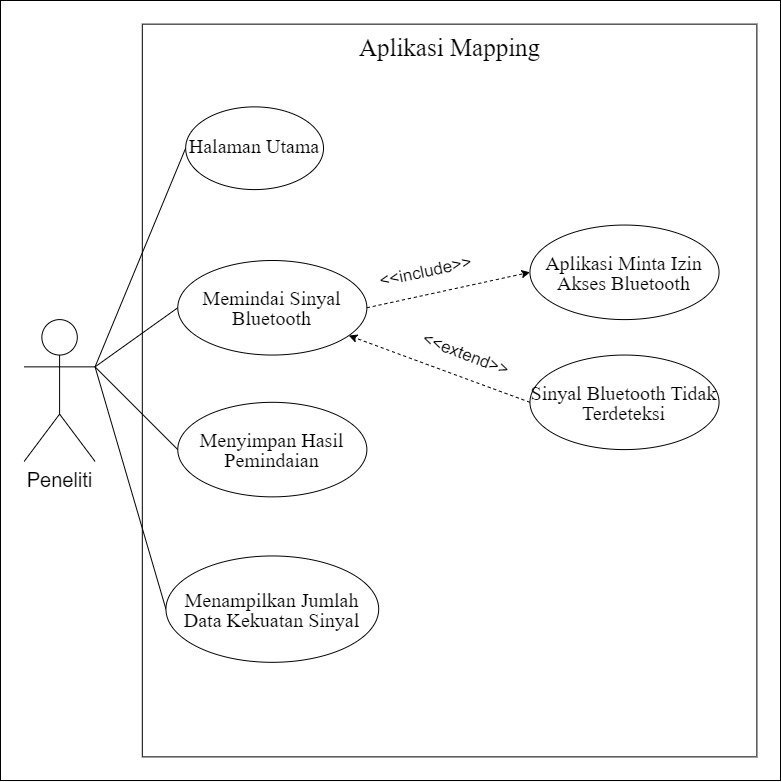
\includegraphics [width=8.5cm, height=8cm]{gambar/mapping}}
	\caption{\textit{Use Case Diagram} Aplikasi Mapping.}
	\label{usecasemapping}
\end{figure}

\par Gambar \ref{usecasemapping} diatas menjelaskan aktivitas yang dapat dilakukan oleh peneliti saat menggunakan aplikasi mapping. Ketika peneliti membuka aplikasi mapping, maka akan muncul halaman beranda. Kemudian, peneliti diminta untuk mengizinkan aplikasi mengakses lokasi pada perangkat. Selanjutnya, peneliti dapat melakukan pemindaian kekuatan sinyal setelah menghidupkan Bluetooth pada perangkat \textit{smartphone}. Setelah itu, hasil dari pemindaian kekuatan sinyal tersebut disimpan didalam server dan dapat ditampilkan jumlah data kekuatan sinyal.
\fancyhf{}
\fancyfoot[R]{\thepage}
\begin{figure}[H]
	\center
	\shadowbox
	{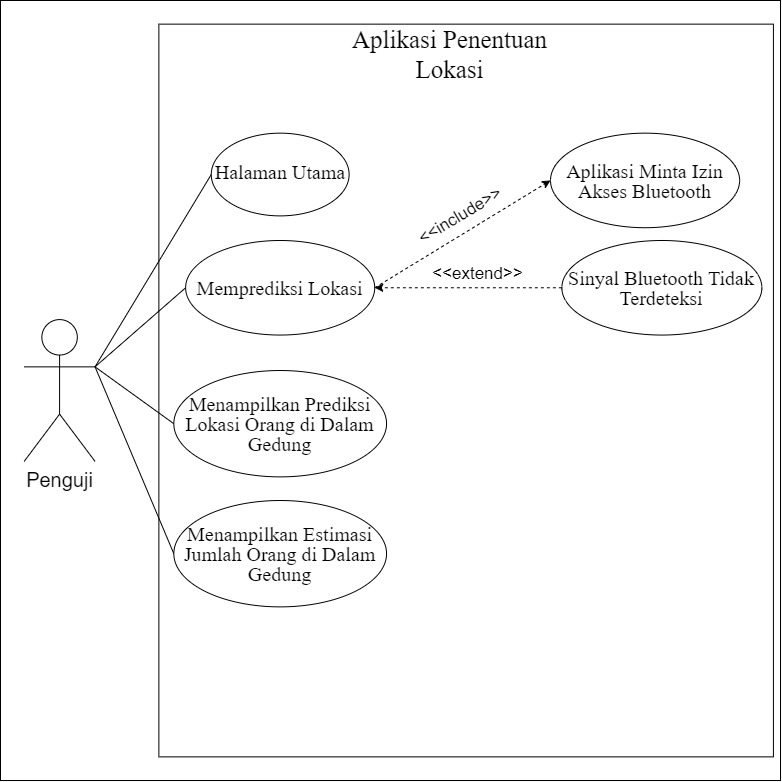
\includegraphics [width=10cm, height=9cm]{gambar/penentuanlokasi}}
	\caption{\textit{Use Case Diagram} Aplikasi LocaLization}
	\label{usecasedosen}
\end{figure}

\par Gambar \ref{usecasedosen} menjelaskan aktivitas yang dapat dilakukan oleh setiap orang yang memasuki gedung Fakultas Matematika dan Ilmu Pengetahuan Alam Universitas Syiah Kuala. Aktivitas pertama yang dapat dilakukan adalah membuka aplikasi LocaLization, pengguna dapat menikmati fitur-fitur yang tersedia seperti melihat estimasi atau jumlah orang yang sedang berada didalam gedung, memulai proses pengecekan lokasi diri sendiri saat berada didalam gedung FMIPA USK dengan syarat keadaan \textit{Bluetooth} pada perangkat dalam keadaan hidup dan melihat kecepatan prediksi berapa detik. Jika pengguna berada diluar gedung FMIPA USK, maka perangkat akan memprediksi pengguna sedang berada diluar jangkauan.

\begin{figure}[H]
	\center
	\shadowbox
	{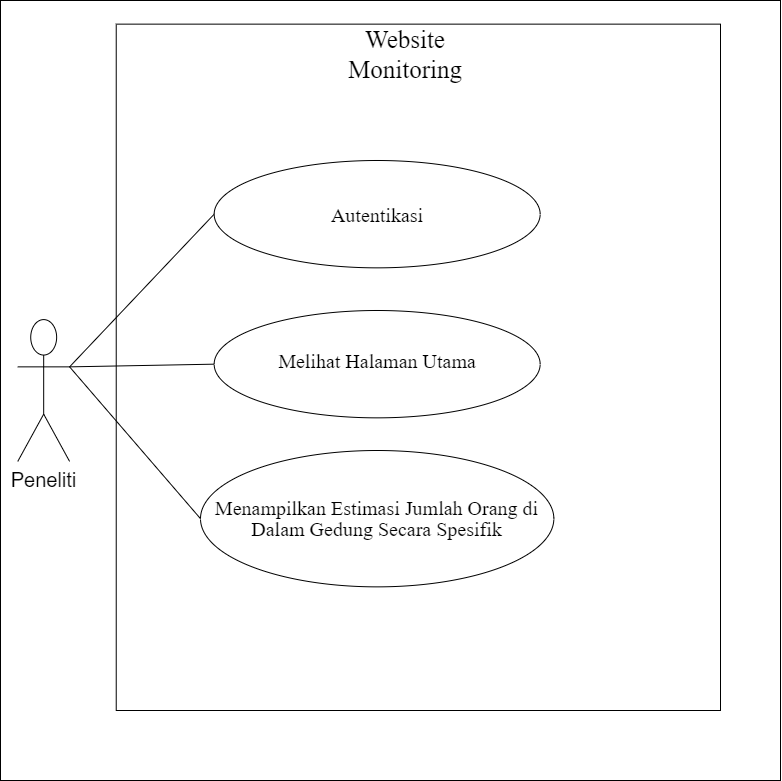
\includegraphics [width=10cm, height=9cm]{gambar/model/usecaseWebMonitoring}}
	\caption{\textit{Use Case Diagram Website Monitoring}.}
	\label{usecasewebmonitoring}
\end{figure}

Gambar \ref{usecasewebmonitoring} menerangkan tentang aktivitas yang dilakukan oleh admin atau peneliti saat  menggunakan website monitoring. Saat peneliti atau admin membuka website monitoring, harus login terlebih dahulu. Setelah itu, akan langsung masuk ke halaman dasbor yang menyajikan data tentang total jumlah orang yang sedang berada di dalam gedung. Di bagian ini, akan menampilkan 2 kolom, untuk kolom pertama menampilan data yang menggunakan algoritma SVM dan kolom kedua menampilkan data yang menggunakan algoritma K-Means. Kemudian di halaman lain, menampilkan data total estimasi orang yang menggunakan aplikasi ini pada tiap posisi di dalam gedung dalam bentuk tabel dan grafik.


% //TODO:Selanjutnya Buat diagram Deployment
\section{PERANCANGAN SISTEM APLIKASI LOCALIZATION}

% \subsection{Perancangan Sistem}

\par Nama LocaLization diberikan untuk nama aplikasi utama berbasis android pada penelitian ini. Perancangan sistem adalah sekumpulan aktivitas yang mendeskripsikan secara rinci bagaimana sistem akan berjalan. Hal itu bertujuan untuk menghasilkan produk perangkat lunak yang sesuai dengan kebutuhan user. Perancangan sistem yaitu rancangan atau susunan sistem yang akan dibangun. Proses ini terdiri dari dua tahap yaitu perancangan konfigurasi eksekusi sistem dalam bentuk \textit{deployment diagram} dan perancangan tampilan antar muka (\textit{interface}).

Tahap pertama adalah merancang \textit{deployment diagram}. \textit{Deployment diagram} adalah diagram yang menjelaskan bagaimana sistem bekerja dan digunakan oleh pengguna. Berikut rancangan \textit{deployment diagram} dari sistem yang telah dibangun dapat dilihat pada Gambar \ref{deployment-diagram}.

%\begin{enumerate}
%\item \textit{Deployment Diagram} Aplikasi Mapping
\vspace{-0.2cm}
\begin{landscape}
	\begin{figure}[H]
		\center
		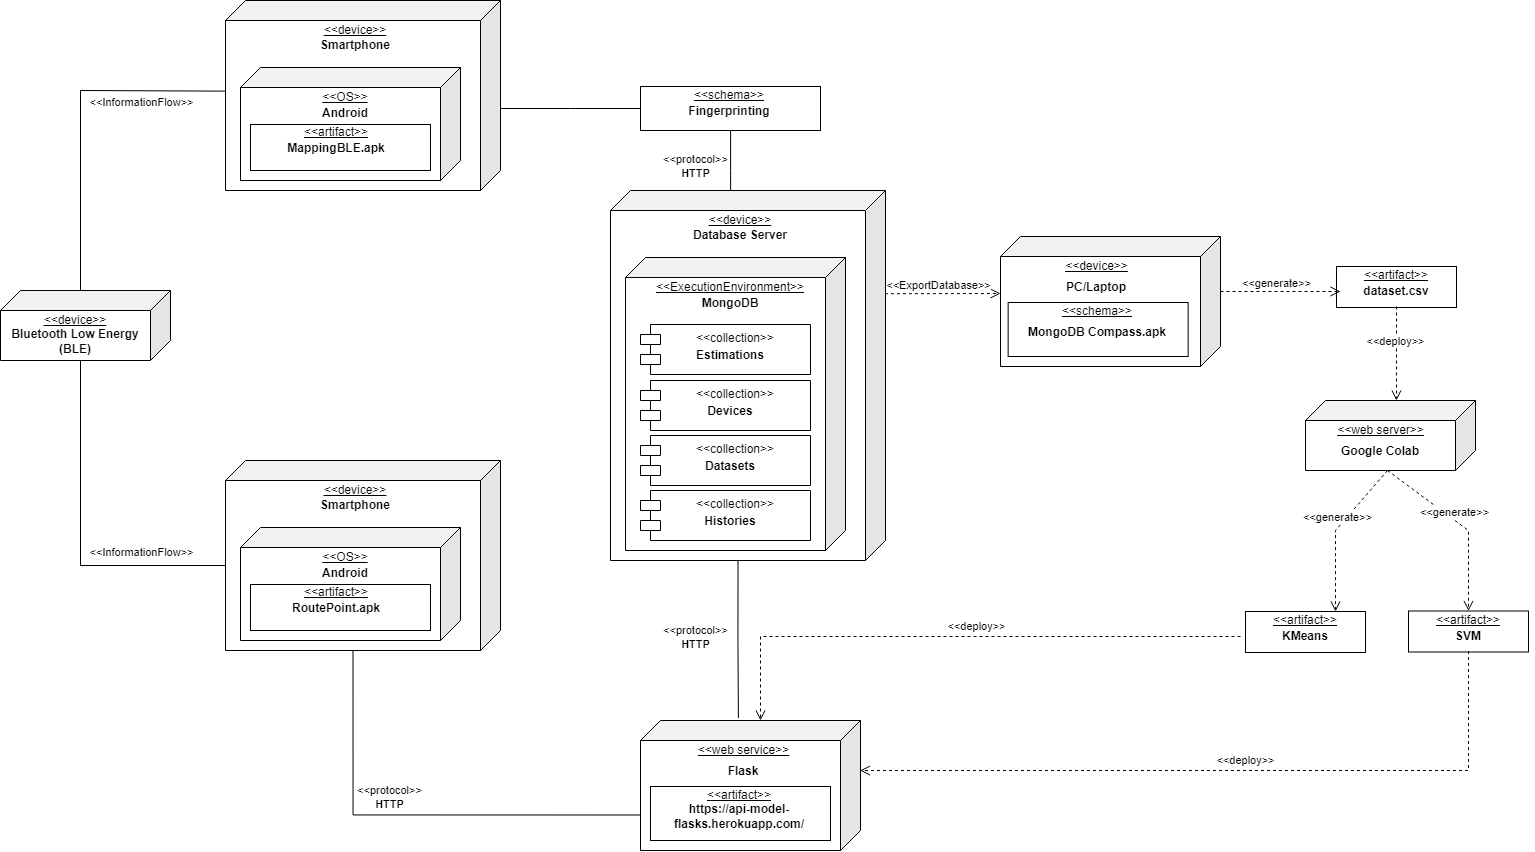
\includegraphics [width = 22.5cm, height=12cm]{gambar/model/diagramdeployment.png}
		\caption{Diagram \textit{Deployment}}
		\label{deployment-diagram}
	\end{figure}
\end{landscape}

Tahap kedua adalah merancang tampilan antar muka pengguna (\textit{user interface}) sebagai mekanisme komunikasi dengan sistem. Antar muka dari sistem yang telah dibangun adalah sebagai berikut:
\begin{enumerate}[a.]

	% \item Antar Muka Aplikasi Mapping
	%       \par Gambar \ref{aplikasimappingbagian1} menampilkan halaman awal ketika aplikasi pertama dibuka, pada halaman ini terdapat fitur untuk memasukkan nama tempat, serta fitur untuk menampilkan informasi   nama \textit{device} Bluetooth, RSSI, dan \textit{MAC address} Bluetooth, Serta pada bagian bawah terdapat empat fitur  yang masing-masing memiliki  fungsi untuk memindai , menampilkan waktu tunggu, menyimpan data dan menampilkan jumlah data yang telah disimpan. Apabila pengguna melakukan pemindaian maka akan muncul notifikasi untuk mengaktifkan Bluetooth. Apabila Bluetooth sudah hidup, maka aplikasi akan mencari nama \textit{device} Bluetooth, RSSI dan dan \textit{MAC address} Bluetooth yang ada di sekitar, pada bagian bawah fitur pemindai akan berubah menjadi stop dan fitur waktu akan menampilkan waktu tunggu  selama 10 detik, waktu ini digunakan  untuk menyamaratakan waktu pemindaian untuk setiap data. Kemudian setelah data disimpan, pada fitur yang menampilkan jumlah data yang telah disimpan yang awalnya 0 sekarang menjadi 1 yang berarti 1 data sudah dimasukkan ke dalam \textit{database server}.

	%   \vspace{-0cm}
	%   \begin{figure} [H]
	%       \begin{subfigure}{.5\textwidth}
	% 	      \centering
	% 	      % include first image
	% 	      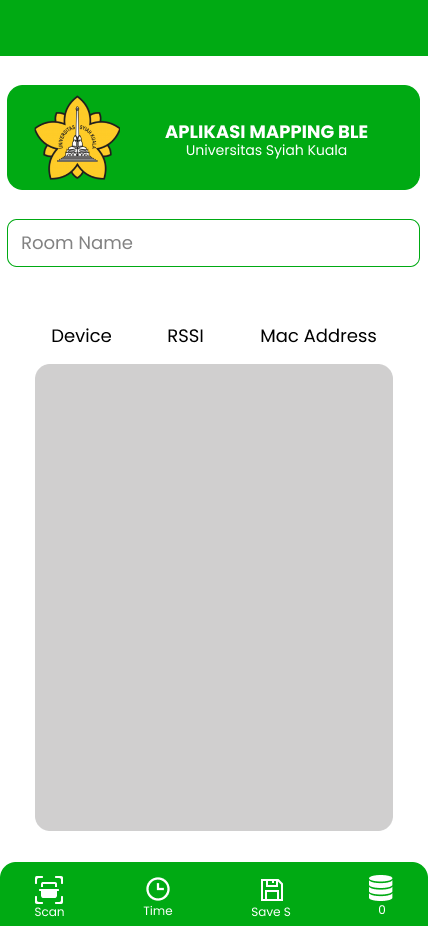
\includegraphics[width=.5\linewidth]{gambar/mapping1.png}
	% 	      \caption{Halaman awal aplikasi \textit{mapping}}
	%       \end{subfigure}
	%       \begin{subfigure}{.5\textwidth}
	% 	      \centering
	% 	      % include second image
	% 	      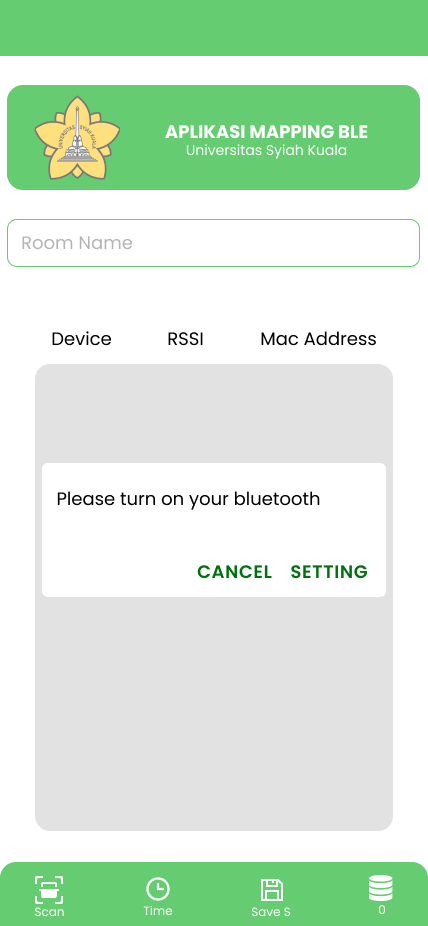
\includegraphics[width=.5\linewidth]{gambar/mapping2.png}
	% 	      \caption{Izin mengakses Bluetooth}
	%       \end{subfigure}
	%       \vspace{1cm}
	%       \newline
	%       \begin{subfigure}{.5\textwidth}
	% 	      \centering
	% 	      % include third image
	% 	      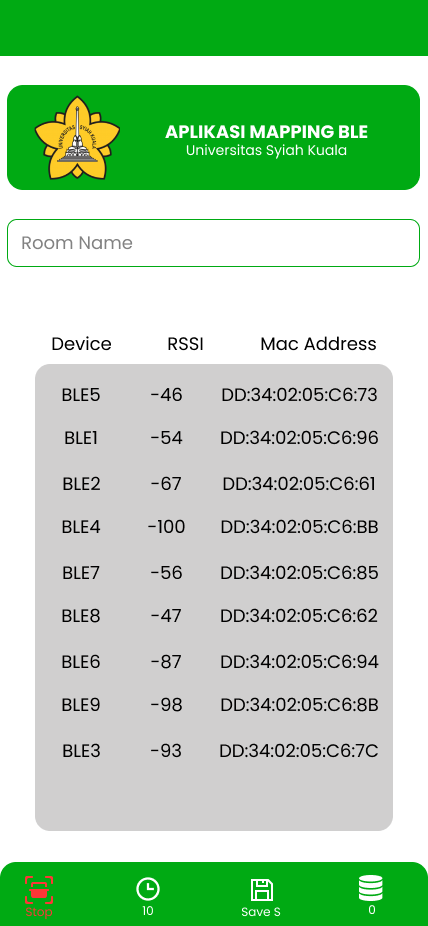
\includegraphics[width=.5\linewidth]{gambar/mapping3.png}
	% 	      \caption{Proses pemindaian kekuatan sinyal}
	%       \end{subfigure}
	%       \begin{subfigure}{.5\textwidth}
	% 	      \centering
	% 	      % include fourth image
	% 	      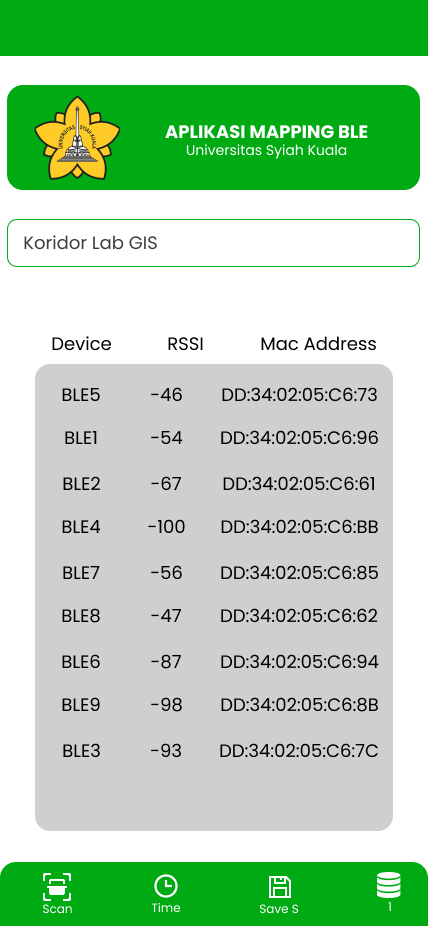
\includegraphics[width=.5\linewidth]{gambar/mapping4.png}
	% 	      \caption{Selesai proses pemindaian}
	%       \end{subfigure}
	%       \vspace{0.5cm}
	%       \caption{Tampilan Halaman Aplikasi Mapping}
	%       \label{aplikasimappingbagian1}
	%   \end{figure}

	% \vspace{1cm}
	\item Antar Muka Aplikasi LocaLization

	      \par Nama LocaLization adalah nama yang diberikan untuk aplikasi utama yang berbasis android pada penelitian ini. Gambar \ref{aplikasiPenentuanLokasi} memperlihatkan halaman awal saat memulai menggunakan aplikasi ini. Di halaman awal setelah splash screen, pengguna akan diajak untuk menggunakan aplikasi ini agar mengetahui informasi estimasi orang dan posisi pengguna di dalam gedung. Setelah itu, akan digiring ke halaman untuk cek lokasi. Pada halaman ini, pengguna akan di minta izin untuk mengambil datanya oleh sistem agar bisa melacak keberadaanya secara anonim dan rahasia. Dengan menekan tombol Cek Lokasi, pengguna akan di anggap memberi izin jika datanya diambil untuk proses \textit{Indoor Localization System}.


	      \vspace{-0cm}
	      \begin{figure} [H]
		      \begin{subfigure}{.5\textwidth}
			      \centering
			      % include first image
			      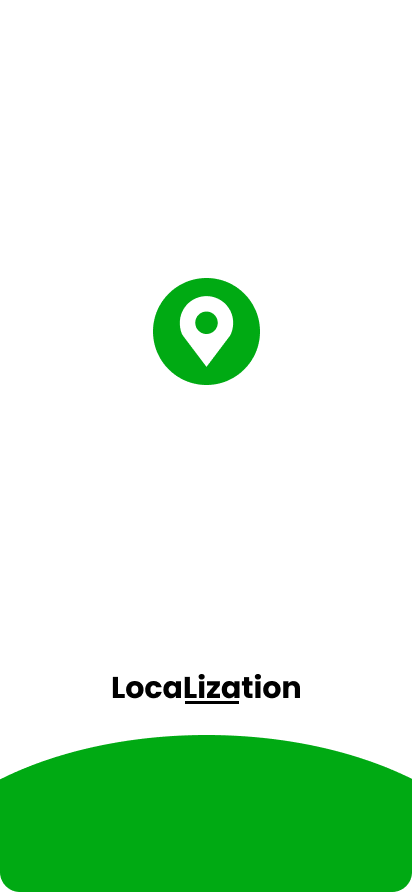
\includegraphics[width=.5\linewidth]{gambar/splashscreen.png}
			      \caption{Halaman Pertama Pembuka Aplikasi}
		      \end{subfigure}
		      \begin{subfigure}{.5\textwidth}
			      \centering
			      % include second image
			      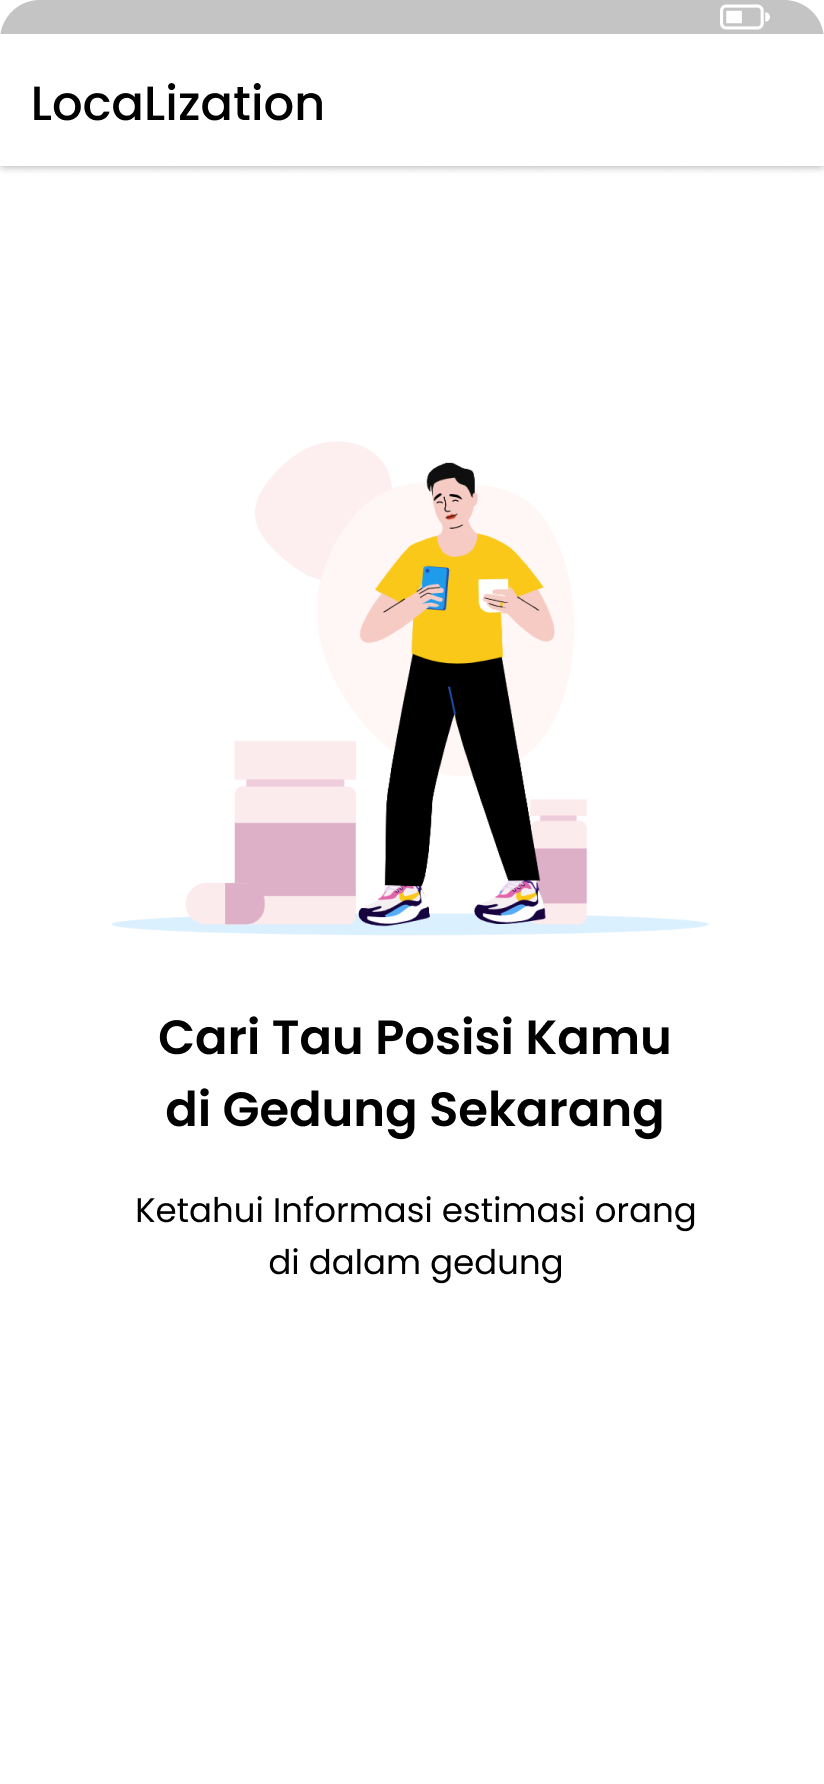
\includegraphics[width=.5\linewidth]{gambar/mulai.png}
			      \caption{Halaman Ajakan Menggunakan Aplikasi}
		      \end{subfigure}
		      \vspace{1cm}
		      \newline
		      \begin{center}
			      \begin{subfigure}{.5\textwidth}
				      \centering
				      % include third image
				      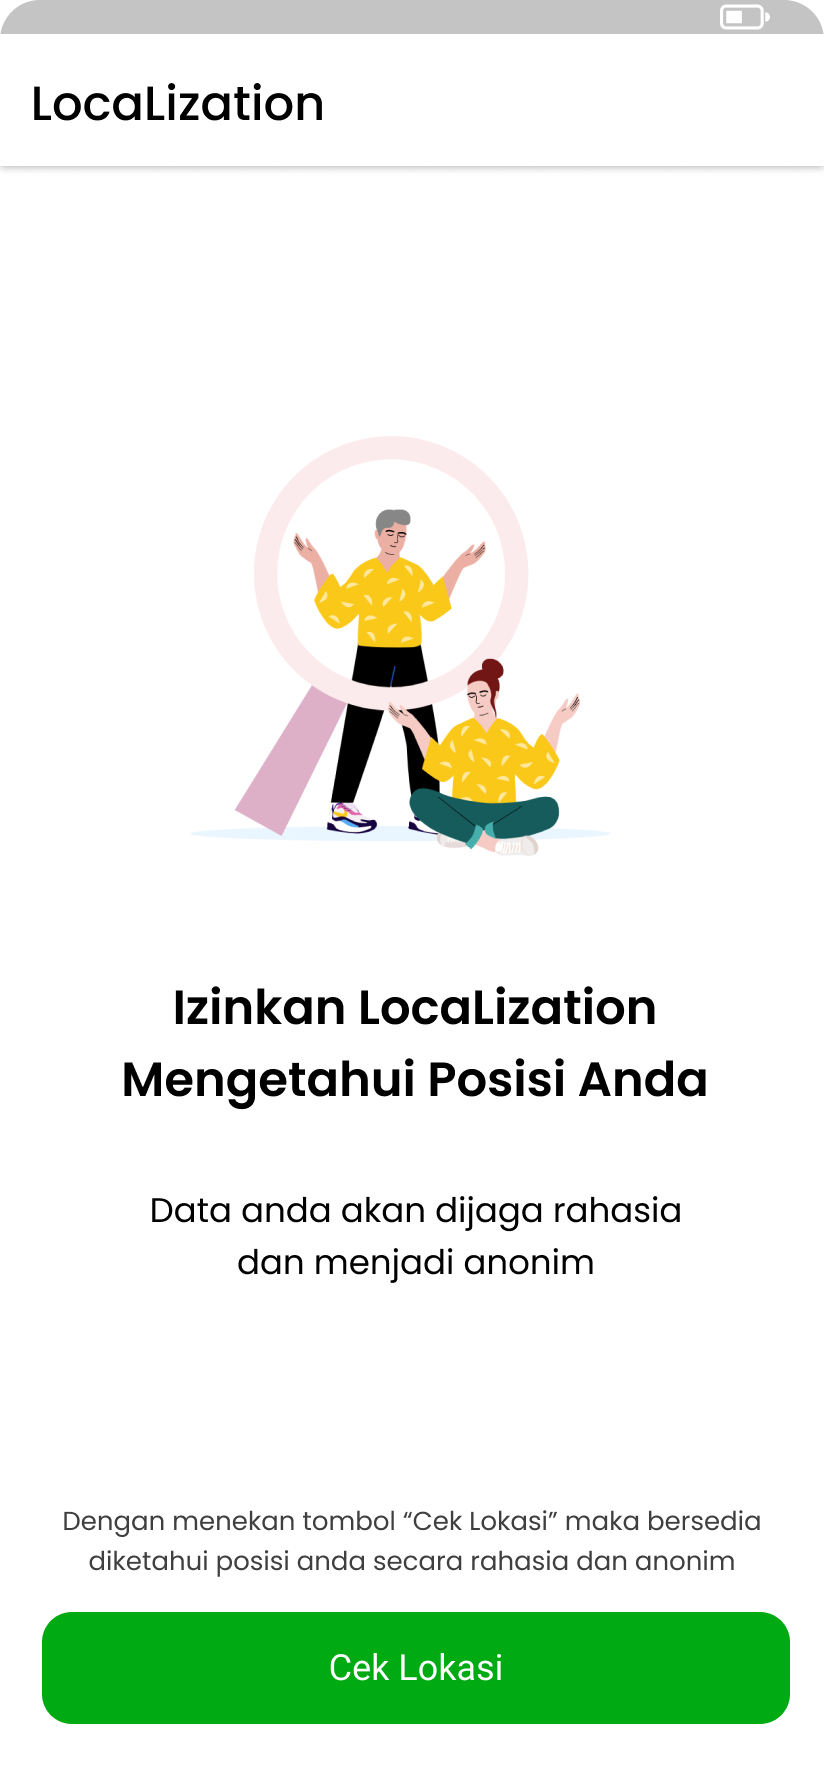
\includegraphics[width=.5\linewidth]{gambar/mulai (1).png}
				      \caption{Halaman untuk Mulai Cek Lokasi}
			      \end{subfigure}
		      \end{center}
		      \vspace{0.5cm}
		      \caption{Tampilan Awal Saat Memulai Menggunakan Aplikasi}
		      \label{aplikasiPenentuanLokasi}
	      \end{figure}

	      \vspace{0.5cm}

	      \par Proses cek lokasi memerlukan sinyal \textit{bluetooth} dan internet. Waktu yang dibutuhkan dalam \textit{scanning} adalah 10 detik. Hasil prediksi akan keluar seperti pada gambar \ref{aplikasiPenentuanLokasi2}

	      \vspace{-0cm}
	      \begin{figure} [H]
		      \begin{subfigure}{.5\textwidth}
			      \centering
			      % include first image
			      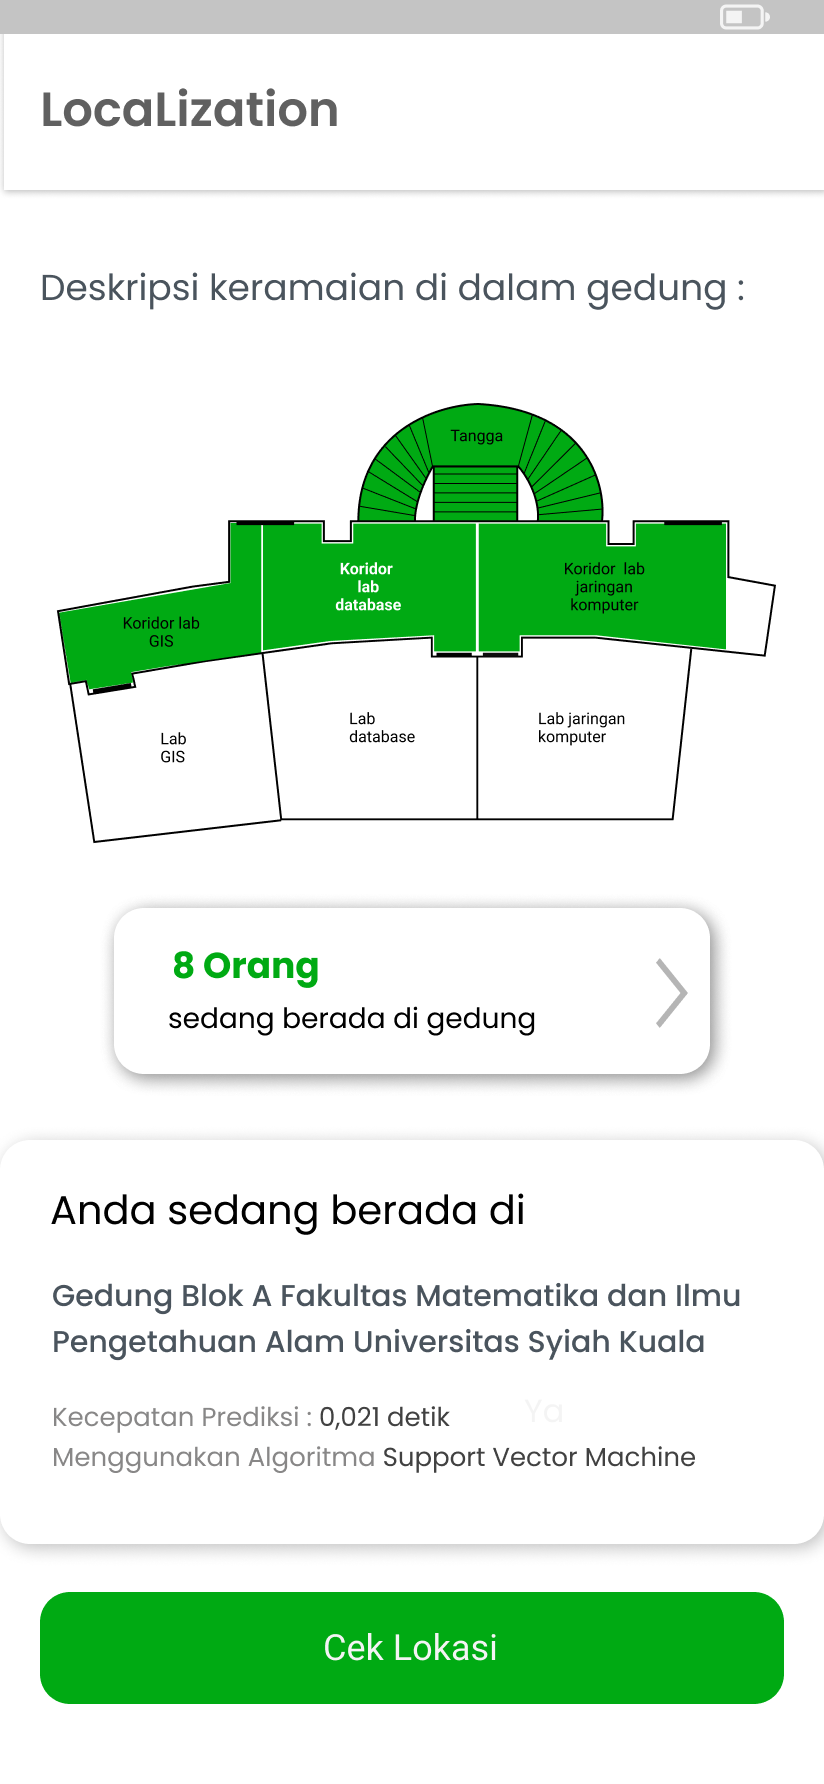
\includegraphics[width=.5\linewidth]{gambar/lantai9(1).png}
			      \caption{Halaman Pertama Pembuka Aplikasi}
		      \end{subfigure}
		      \begin{subfigure}{.5\textwidth}
			      \centering
			      % include second image
			      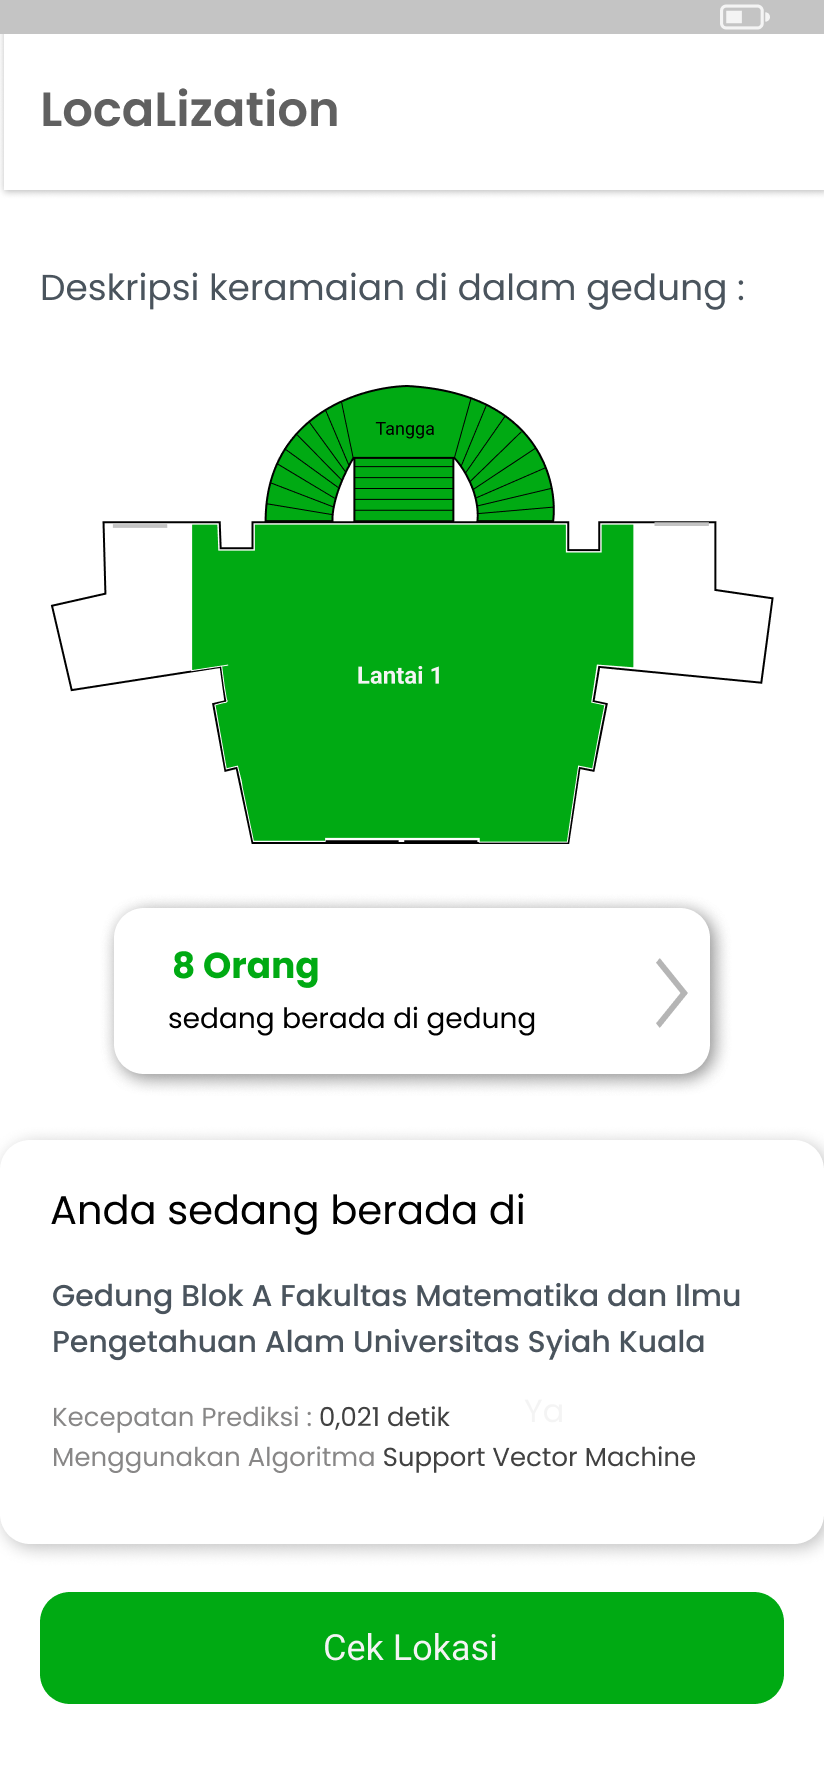
\includegraphics[width=.5\linewidth]{gambar/lantai4(1).png}
			      \caption{Halaman Ajakan Menggunakan Aplikasi}
		      \end{subfigure}
		      \vspace{1cm}
		      \newline
		      \begin{center}
			      \begin{subfigure}{.5\textwidth}
				      \centering
				      % include third image
				      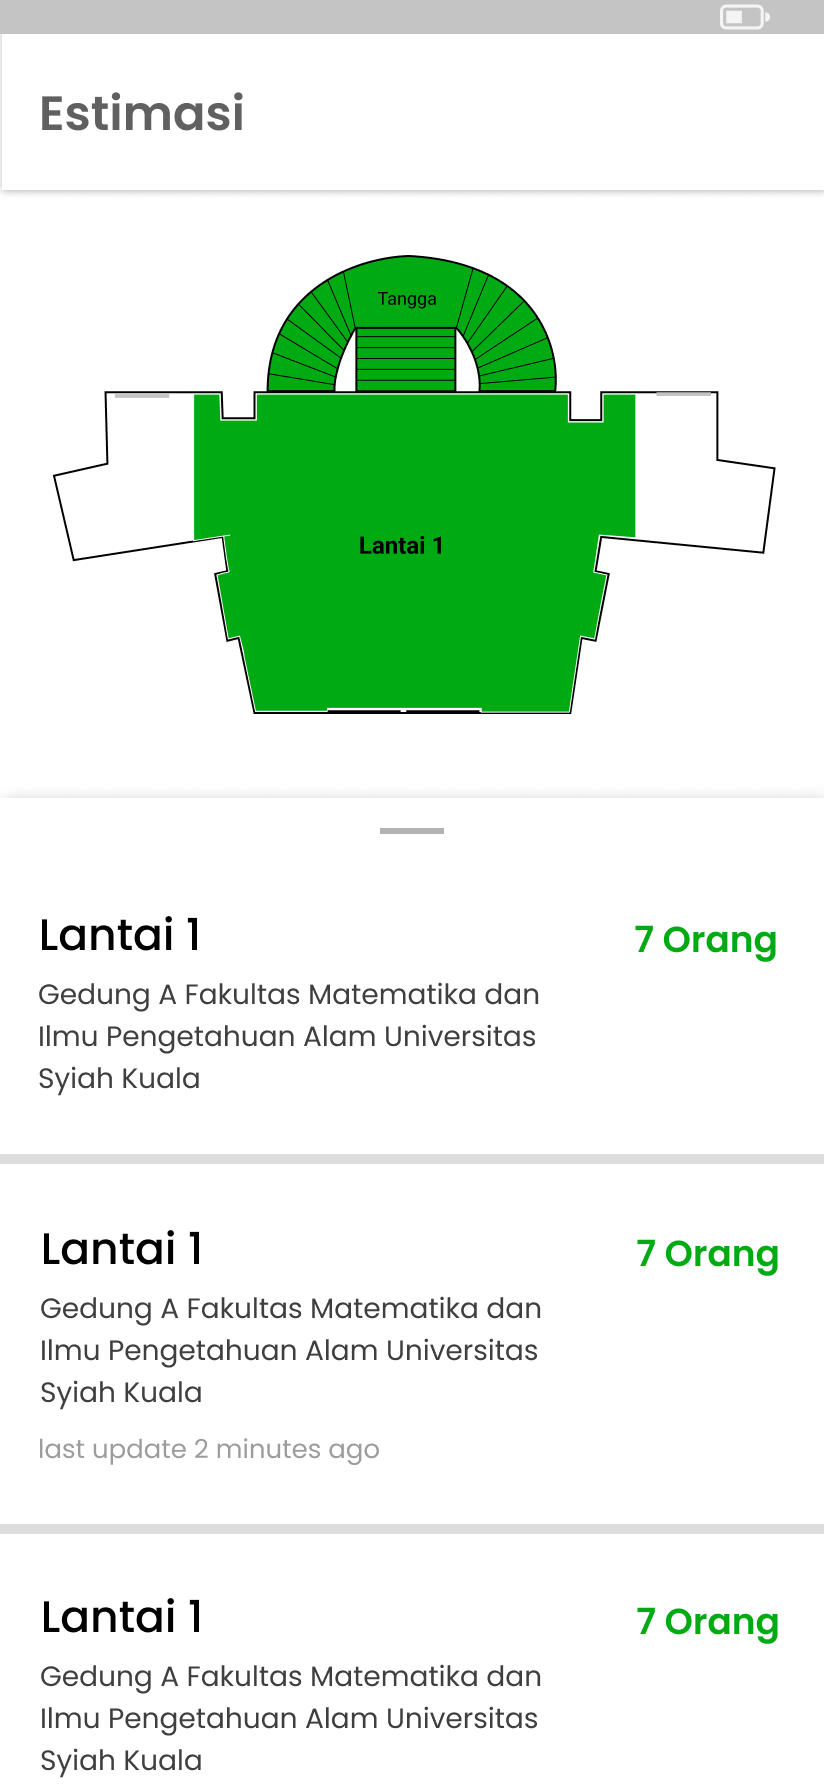
\includegraphics[width=.5\linewidth]{gambar/lantai8(1).png}
				      \caption{Halaman untuk Mulai Cek Lokasi}
			      \end{subfigure}
		      \end{center}
		      \vspace{0.5cm}
		      \caption{Tampilan Awal Saat Memulai Menggunakan Aplikasi}
		      \label{aplikasiPenentuanLokasi2}
	      \end{figure}

	      \vspace{0.5cm}

	\item Antar Muka Aplikasi Web Monitoring

	      \par Gambar \ref{LoginWeb} adalah halaman login untuk pengguna aplikasi \textit{web monitoring} yaitu peneliti dan admin. Setelah login, maka peneliti atau admin langsung masuk ke halaman dasbor, seperti pada gambar \ref{Dashbord}. Pada halaman dasbor akan ditampilkan informasi data estimasi orang di dalam gedung dalam 2 kolom. Kolom pertama menampilkan data hasil dari algoritma SVM dan kolom kedua menampilkan data hasil dari algoritma K-Means. Selain halaman dasbor, ada halaman yang menampilkan informasi data estimasi tiap posisi yang di dalam gedung dalam bentuk grafik dan dalam bentuk tabel. Contohnya dapat dilihat pada gambar \ref{Estimasi_Grafik} dan gambar \ref{Estimasi_Tabel}


	      \vspace{-0cm}
	      \begin{figure}[H]
		      \center
		      \includegraphics [width = 13.5 cm, height= 6.75 cm]{gambar/web/Login}
		      \caption{Halaman \textit{login}Web Monitoring}
		      \label{LoginWeb}
	      \end{figure}
	      \begin{figure}[H]
		      \center
		      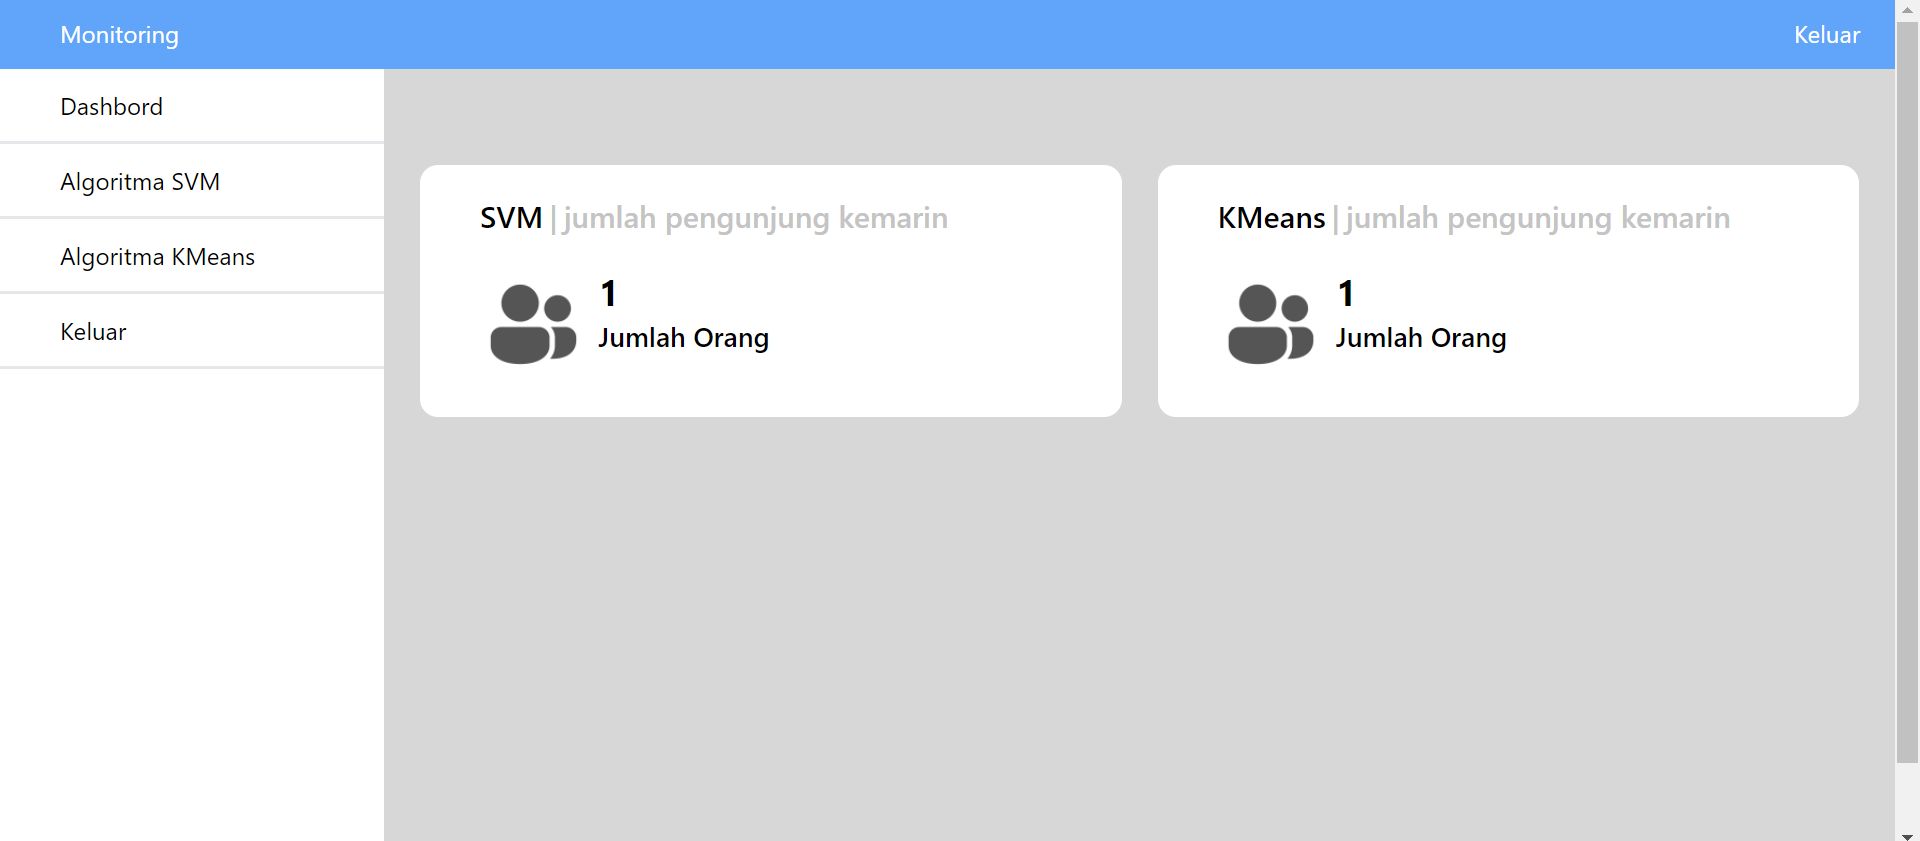
\includegraphics [width = 13.5 cm, height= 6.75 cm]{gambar/web/Dashbord}
		      \caption{Halaman \textit{dashbord}}
		      \label{Dashbord}
	      \end{figure}
	      \begin{figure}[H]
		      \center
		      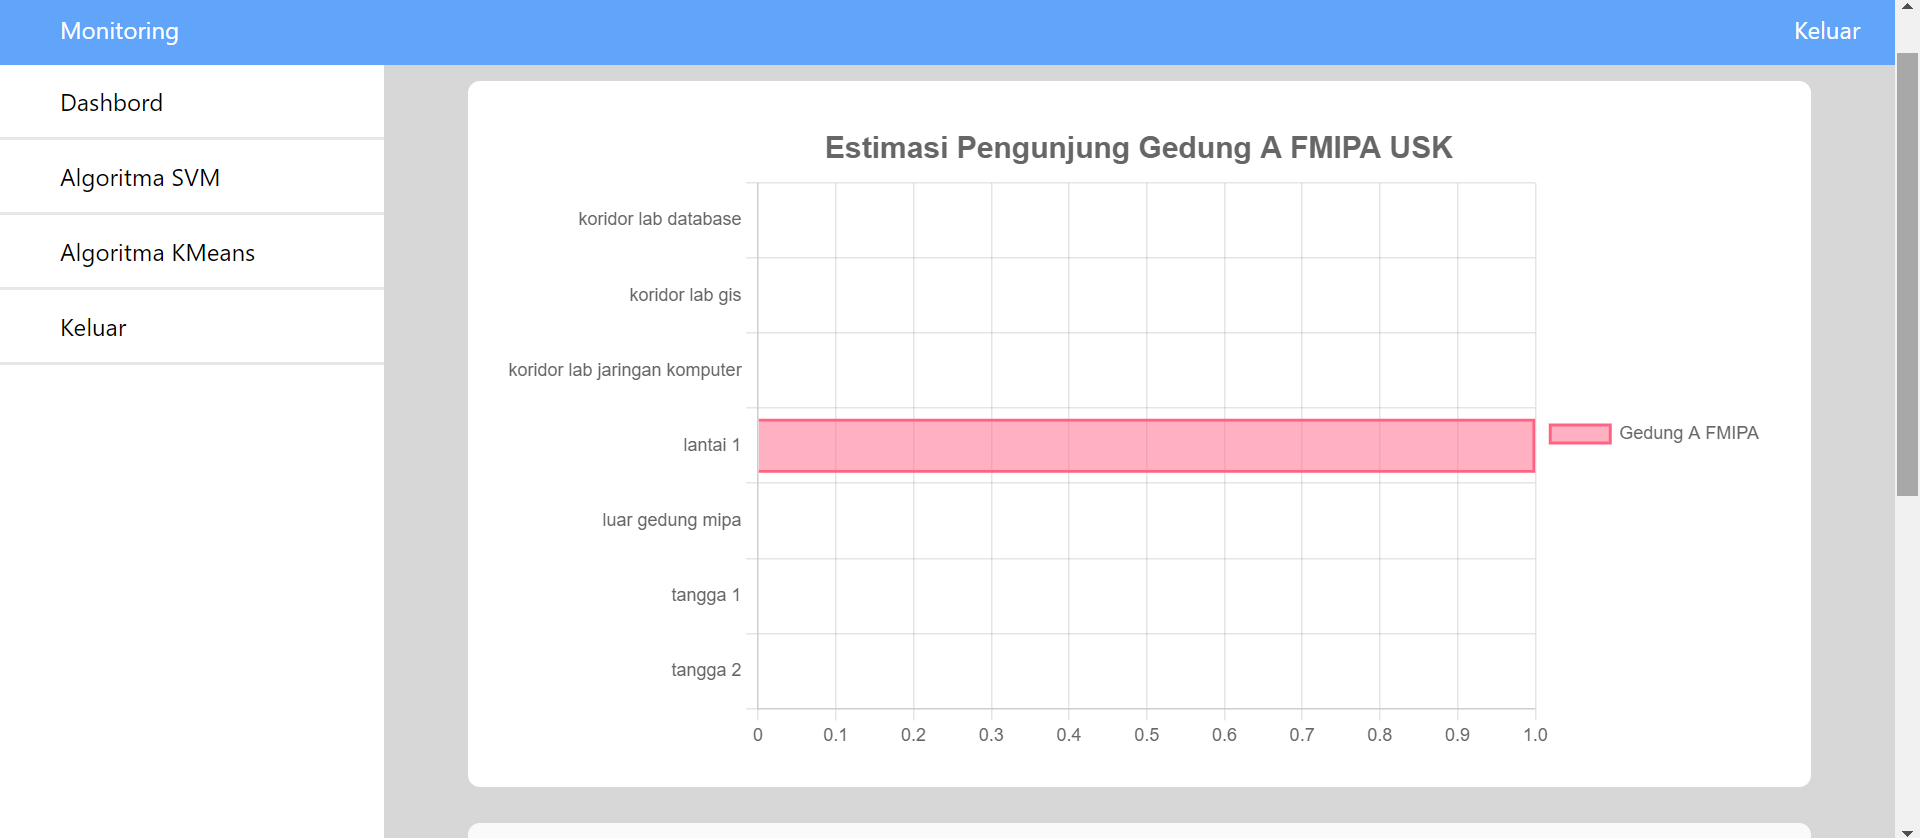
\includegraphics [width = 13.5 cm, height= 6.75 cm]{gambar/web/Estimasi_Grafik}
		      \caption{Halaman Estimasi Orang Tiap Posisi dalam Bentuk Grafik}
		      \label{Estimasi_Grafik}
	      \end{figure}
	      \begin{figure}[H]
		      \center
		      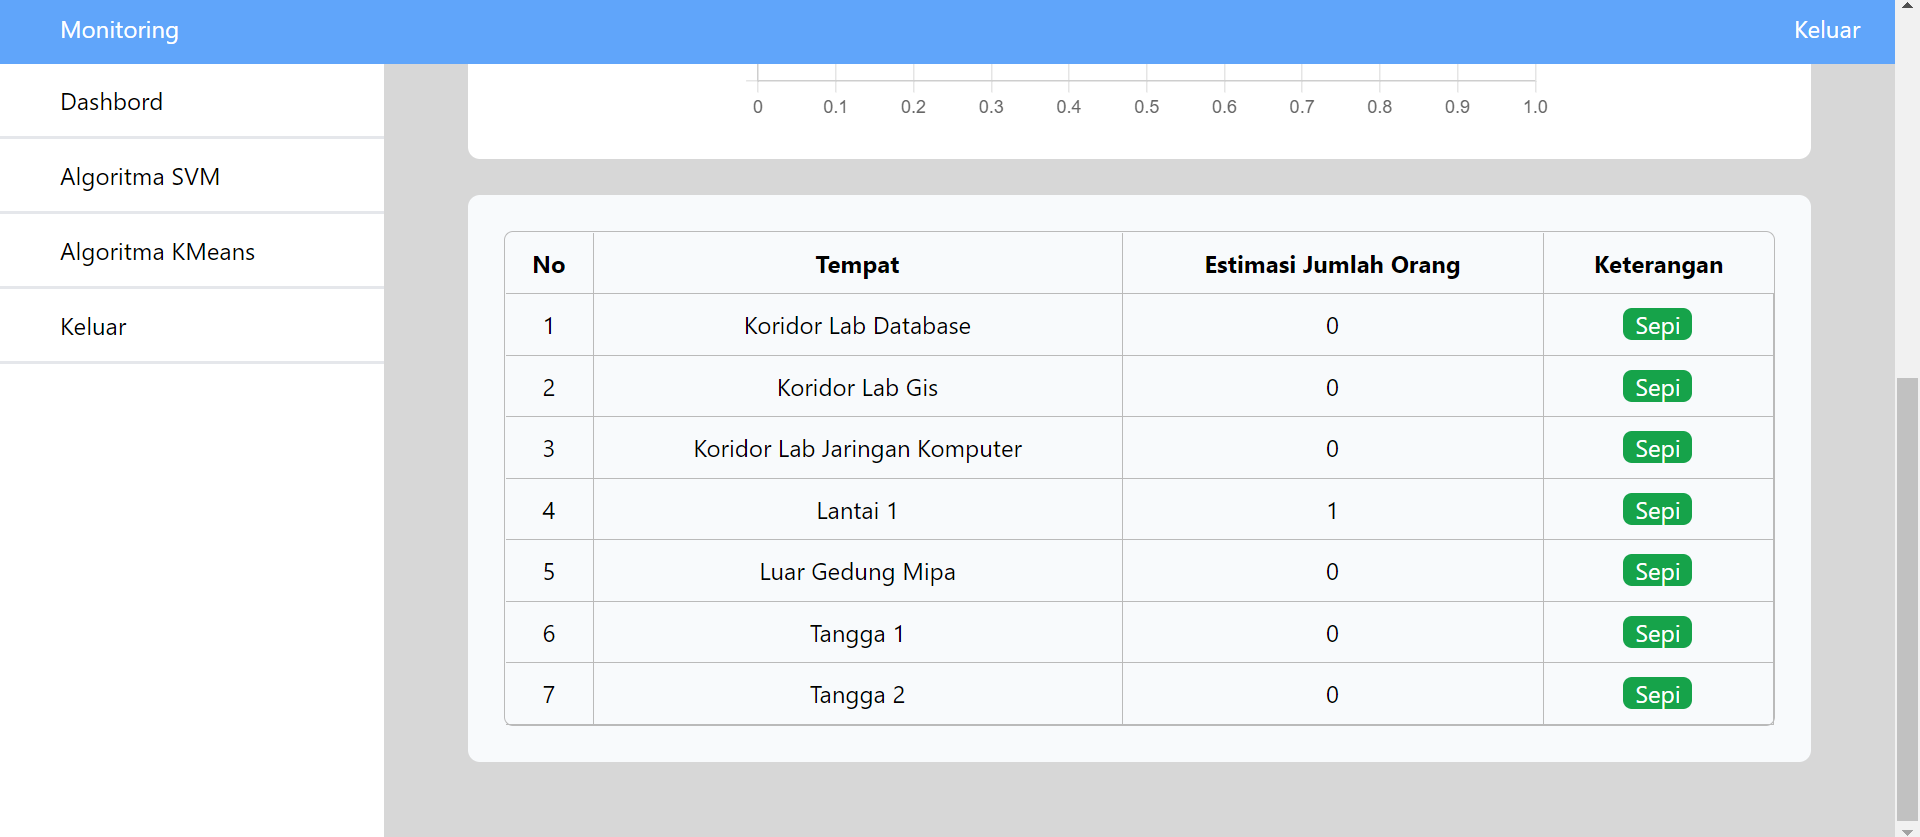
\includegraphics [width = 13.5 cm, height= 6.75 cm]{gambar/web/Estimasi_Tabel}
		      \caption{Halaman Estimasi Orang Tiap Posisi dalam Bentuk Tabel}
		      \label{Estimasi_Tabel}
	      \end{figure}
\end{enumerate}

%%%%%%%%%%%%%%%%%%%%%%%%%%%%%%%%%%%%%%%%%%%akhir perancangan aplikasi mapping%%%%%%%%%%%%%%%%%%%%%%%%%%%%%%%%%%%%%%%%%%%%%%%%%%%
% \subsection{Pembuatan Sistem}

% \begin{enumerate}[a.]
% \item Aplikasi \textit{Mapping}
%       \\ Aplikasi \textit{mapping} merupakan  aplikasi \textit{mobile} berbasis Android yang dibuat menggunakan bahasa pemrograman JavaScript dengan \textit{framework} React Native. Media untuk penyimpanan data pada aplikasi \textit{mapping} ini menggunakan \textit{database} MongoDb Compass yang datanya akan dikirim melalui \textit{Web Service}. Potongan kode program yang terdapat dalam aplikasi \textit{mapping} ini dapat dilihat pada Progran 4.1 berikut ini.
%       \vspace{0.4cm}
%       \lstset{language=Java,
% 	      basicstyle=\ttfamily\scriptsize\color{black},
% 	      keywordstyle=\color{javapurple}\bfseries,
% 	      stringstyle=\color{javared},
% 	      commentstyle=\color{javagreen},
% 	      morecomment=[s][\color{javadocblue}]{/**}{*/},
% 	      numbers=left,
% 	      numberstyle=\tiny\color{black},
% 	      showstringspaces=false,
% 	      numbersep=10pt,
% 	      tabsize=4,
% 	      showspaces=false,
% 	      showstringspaces=false,
% 	      autogobble=true,
% 	      xleftmargin=2em
%       }
%       \begin{lstlisting}[label=programScanBle]
% 		import React, { useState } from 'react';
% 		import {
% 			Image,StyleSheet,Text,FlatList,View,TouchableOpacity,Alert,
% 		} from 'react-native';
% 		import { ScrollView, TextInput } from 'react-native-gesture-handler';
% 		import { manager } from '../Ble';
% 		import AkunSvg from './../svg/AkunSvg';
% 		import { colors, sizes } from '../constants';
% 		import Card from '../components/Card';
% 		import Table from './../components/Table';
% 		import BottomNav from '../components/BottomNav';

% 		const HomeScreen = () => {
% 		  const [showData, setShowData] = useState<any[]>([]);
% 		  const [label, setLabel] = useState<string>('');
% 		  const handleDevices = (devices: any) => {
% 			setShowData(devices);
% 		  };
% 		  const renderItem = ({ item, index }: any) => (
% 			<View style={styles.dataTable} key={index}>
% 			  <Text style={[{ width: '40%' }]}>{item.name}</Text>
% 			  <Text style={[{ width: '20%' }]}>{item.rssi}</Text>
% 			  <Text style={[{ width: '40%' }]}>{item.macAddress}</Text>
% 			</View>
% 		  );
% 		  return (
% 			<View style={styles.container}>
% 			  <View style={styles.header}>
% 				<Text></Text>
% 			  </View>

% 			  <Card />

% 			  <View>
% 				<TextInput
% 				  style={styles.formInput}
% 				  placeholder={'Room Name'}
% 				  onChangeText={(value) => setLabel(value)}
% 				  value={label}
% 				/>
% 			  </View>

% 			  <View style={styles.tableContainer}>
% 				<View style={styles.headerTable}>
% 				  <Text style={[{ width: '40%' }]}>Devices</Text>
% 				  <Text style={[{ width: '20%' }]}>RSSI</Text>
% 				  <Text style={[{ width: '40%' }]}>Mac Address</Text>
% 				</View>

% 				{showData.length === 0 ? (
% 				  <ScrollView style={styles.listContainer}></ScrollView>
% 				) : (
% 				  <ScrollView style={styles.listContainer}>
% 					{showData.map((item, index) => {
% 					  return renderItem({ item, index });
% 					})}
% 				  </ScrollView>
% 				)}
% 			  </View>

% 			  <BottomNav onSetData={handleDevices} label={label} />
% 			</View>
% 		  );
% 		};

% 		export default HomeScreen;
% \end{lstlisting}
%       \captionof{lstlisting}{Potongan Kode Program dalam aplikasi \textit{mapping}.}


% 	\item Aplikasi LocaLization Berbasis Android
% 	      \\
% 	      Aplikasi ini adalah aplikasi utama yang berbasis Android dan dibuat menggunakan bahasa pemrograman JavaScript dengan \textit{framework} React Native. Aplikasi ini akan memindai sinyal RSSI yang di pancar dari tiap BLE yang dipasang di setiap sudut ruangan. Waktu yang dibutuhkan untuk memindai sinyal RSSI adalah 10 detik, kemudian data sinyal RSSI tersebut akan dikirim ke API [isi nanti]. Di dalam API tersebut, terdapat model yang sudah dibuat sebelumnya menggunakan algoritma \textit{Support Vector Machine} (SVM). Setelah itu, API akan mengirimkan hasil prediksi lokasi saat ini dari model ke aplikasi utama yaitu aplikasi berbasis Android tadi. Aplikasi LocaLization berbasis Android ini akan menampilkan hasil prediksi total estimasi jumlah orang dan detail estimasi orang di tiap posisi di dalam gedung A FMIPA USK.

% 	\item Aplikasi Web Monitoring
% 	      \\ Aplikasi ini akan memonitoring ....

% \end{enumerate}

\section{PENGUMPULAN DATA SINYAL DENGAN APLIKASI \textit{MAPPING}}
\par Proses pengumpulan data di lakukan menggunakan aplikasi pendukung yaitu aplikasi \textit{mapping}. Pada proses ini, dilakukan proses mengumpulkan data sinyal RSSI dari setiap BLE yang di pasang di setiap sudut ruangan di dalam gedung A FMIPA USK. Pada proses ini juga di bantu oleh beberapa orang dengan \textit{device} yang berbeda. Adapun daftar peserta pengumpulan data beserta \textit{device} yang digunakan dapat dilihat sebagai berikut
\begin{table}[H]
	\center
	\fontsize{10}{12}\selectfont
	\caption{Daftar Peserta Pengumpulan Data}
	\label{Daftar-Peserta-Pengumpula-Data}
	\begin{tabular}{|c|l|l|l|c|}
		\hline
		No. & \multicolumn{1}{c|}{\textbf{Nama}}                             & \multicolumn{1}{c|}{\textbf{\textit{Device} yang Digunakan}}   \\ \hline
		1.  & \begin{tabular}[c]{@{}l@{}}Indra Azari\end{tabular}            & \begin{tabular}[c]{@{}l@{}}POCO X3\end{tabular}                \\ \hline
		2.  & \begin{tabular}[c]{@{}l@{}}Aqil Fiqran Dzi'ul Haq\end{tabular} & \begin{tabular}[c]{@{}l@{}}OPPO R7SF\end{tabular}              \\ \hline
		3.  & \begin{tabular}[c]{@{}l@{}}Liza Maiyuni\end{tabular}           & \begin{tabular}[c]{@{}l@{}}SAMSUNG A30\end{tabular}            \\ \hline
		4.  & \begin{tabular}[c]{@{}l@{}}Yaumil Aghnia\end{tabular}          & \begin{tabular}[c]{@{}l@{}}SAMSUNG GALAXY A6 PLUS\end{tabular} \\ \hline
		5.  & \begin{tabular}[c]{@{}l@{}}Atika Fadhluna\end{tabular}         & \begin{tabular}[c]{@{}l@{}}XIAOMI REDMI NOTE 5\end{tabular}    \\ \hline
		6.  & \begin{tabular}[c]{@{}l@{}}Abi Farhan\end{tabular}             & \begin{tabular}[c]{@{}l@{}}XIAOMI REDMI NOTE 5\end{tabular}    \\ \hline
		7.  & \begin{tabular}[c]{@{}l@{}}Ivan Horatius\end{tabular}          & \begin{tabular}[c]{@{}l@{}}OPPO F1+\end{tabular}               \\ \hline
	\end{tabular}

\end{table}

\par Proses pengumpulan data ini menggunakan aplikasi \textit{mapping} dan wajib mengaktifkan internet dan \textit{bluetooth}. Adapun tempat yang digunakan dalam proses ini adalah gedung A FMIPA USK yaitu dari lantai 1 ke lantai 3. Proses ini dilakukan beberapa kali agar data yang didapatkan berkualitas dan jumlahnya banyak.
\par Data sinyal yang berhasil dikumpulkan adalah sebanyak 2049 data dengan jumlah atribut sebanyak 31 atribut dan jumlah label sebanyak 6 label. Adapun atribut pada data sinyal ini adalah data dari setiap beacon sebanyak 31 beacon dan 6 label dari masing-masing posisi di dalam gedung A FMIPA USK. 6 label pada data ini adalah lantai 1, tangga 1 (tangga yang menghubungkan lantai 1 dan 2), tangga 2 (tangga yang menghubungkan lantai 2 dan 3), koridor lab database, koridor lab GIS, dan koridor lab jaringan.

\section{PENGUJIAN AKURASI DENGAN ALGORITMA SVM}

\par Algoritma SVM dibuat dengan menggunakan kode Python dengan memanfaatkan Google Colab. Adapun langkah dalam pengujian  akurasi dengan algoritma SVM adalah sebagai berikut:

\begin{enumerate} [1.]
	\item Visualisasi Data
	      \\ Proses ini menampilkan Visualisasi data sinyal beserta labelnya. Potongan program kode python untuk proses ini dapat dilihat pada Progran 4.1 berikut ini.
	      \\
	      \begin{lstlisting}[label=MinMAxdanPCA,language=Python]
dataset = pd.read_csv("/content/drive/MyDrive/Colab Notebooks/datasets.csv",",")

bankdata = dataset.loc[:,dataTes]
# bankdata = dataset

bankdata.shape

bankdata.head()
					\end{lstlisting}
	      \captionof{lstlisting}{Potongan Kode Program Proses Visualisasi Data Klasifikasi}
	\item Pembuatan File
	      \\Proses ini akan menghasilkan file \textit{pickle} menggunakan algoritma SVM. Adapun contoh potongan kode Pythonnya seperti berikut:

	      \begin{lstlisting}[label=MinMAxdanPCA,language=Python]
import pickle
pickle.dump(svclassifier, open( "model_svm_9", "wb" ))

svclassifier = pickle.load(open( "model_svm_9", 'rb'))
		  \end{lstlisting}
	      \captionof{lstlisting}{Potongan Kode  Proses Pembuatan File Menggunakan SVM}

	\item Pengujian Akurasi
	      \\Perhitungan akurasi algoritma SVM dilakukan dengan cara membagi jumlah data yang diklasifikasikan secara benar dengan total sampel data yang diuji, dengan rumus sebagai berikut:

	      \begin{equation}
		      Akurasi = \frac{Jumlah Benar Diklasifikasi}{Total Data}\times100\%
	      \end{equation}

	      \par Jumlah Benar Diklasifikasi adalah jumlah data testing yang diklasifikasikan secara benar sesuai dengan labelnya lalu dibagi dengan jumlah total data. Pada penelitian ini, ada 1926 data yang diklasifikasikan secara benar dan dibagi dengan total data yang ada. Hasil yang di dapat adalah sebesar 94\%.

	      \begin{center}
		      $Akurasi = \frac{1926}{2048}\times100\%$\\
		      $Akurasi = 94\%$
	      \end{center}


	      \begin{lstlisting}[label=classifier,language=Python]
from sklearn.model_selection import train_test_split
X_train, X_test, y_train, y_test = train_test_split(X, y, test_size = 0.20)

from sklearn.svm import SVC
svclassifier = SVC(kernel='linear')
svclassifier.fit(X_train, y_train)

y_pred = svclassifier.predict(X_test)

from sklearn.metrics import classification_report, confusion_matrix
print(confusion_matrix(y_test,y_pred))
print(classification_report(y_test,y_pred))
\end{lstlisting}
	      \captionof{lstlisting}{Potongan Kode Program Proses Pengujian Akurasi}
\end{enumerate}

\section{PEMBUATAN SISTEM}
\par Proses pembuatan sistem adalah tahapan implementasi dari hasil rancangan sebelumnya. Aplikasi-aplikasi yang akan dibuat adalah sebagai berikut:
\begin{enumerate}[1.]
	\item API Algoritma SVM
	      \par Bahasa pemrograman yang digunakan dalam membangun API ini adalah bahasa Python dengan menggunakan \textit{framework} Flasks.  Api ini dihubungkan dengan database MongoDb untuk menyimpan data. Api ini memiliki beberapa proses sebagai berikut:
	      \begin{enumerate}[a.]
		      \item Menyimpan file hasil algoritma SVM
		            \par Proses ini menyimpan file yang sudah di buat sebelumnya menggunakan algoritma SVM. API mengirimkan hasil klasifikasi dari file ke aplikasi utama. Potongan program kode python untuk proses ini dapat dilihat sebagai berikut:
		            \begin{lstlisting}[language=Python]
@app.route('/api/svm', methods=['GET', 'POST'])
@cross_origin()
def svm():
filename = 'model/model14122021/model_svm'
						
model = pickle.load(open(filename, 'rb'))
						
data = request.form.getlist('data')
if len(data) == 0:
start = time.time()
label = model.predict([[-23, -56, -110, -110, -110, -110, -110, -110, -110, -110, -110, -96,	-100,	-97,	-90,	-90,	-93,	-89,	-95,	-95, -85,	-78,	-95,	-95,	-88, -95,	-110,	-110,	-110,	-110,	-110]]).tolist()[0]
end = time.time()
return {'label': label, 'runtime': end - start}
if len(data) < 31:
return {'type': 'danger', 'message': 'data features tidak boleh dibawah 20'}
if len(data) > 31:
return {'type': 'danger', 'message': 'data features tidak boleh diatas 20'}	

start = time.time()
dataset = [int(row) for row in data]
label = model.predict([dataset]).tolist()[0]
end = time.time()
return {'label': label, 'runtime': end - start}				
								\end{lstlisting}

		      \item Menyimpan Estimasi Jumlah Orang
		            \par Pada proses ini, akan menyimpan data estimasi orang di dalam gedung A FMIPA USK. Apabila seseorang di prediksi berada di dalam gedung A FMIPA, maka akan dihitung bertambah 1 dan sebaliknya jika diprediksi berada di luar gedung A FMIPA, maka tidak dihitung ke dalam estimasi jumlah orang. Total estimasi secara keseluruhan dan detail informasi estimasi akan dikirim ke aplikasi utama yaitu aplikasi berbasis android atau aplikasi LocaLization. Potongan kode untuk proses menambah estimasi dapat dilihat pada program 4.4 sedangkan potongan kode untuk mengurangkan estimasi orang dapat dilihat pada program 4.5.
		            \begin{lstlisting}[language=Python]
@app.route('/api/estimasi/masuk', methods=['POST'])
@cross_origin()
def masukEstimasi():
	algoritma = request.form.get('algoritma')
	label = request.form.get('label').replace(' ', '_').lower()
	currentEstimasi = db.estimations.find_one({'name': algoritma})
	now = datetime.now(pytz.timezone('Asia/Jakarta'))
	current_time = now.strftime("%m/%d/%Y, %H:%M:%S")
	if label in currentEstimasi:
		db.estimations.update_one(
			{'name': algoritma}, {'$set': {'total': currentEstimasi['total'] + 1, label: currentEstimasi[label] + 1, label+'_time': current_time, 'total_time': current_time}})
		return jsonify(algoritma=algoritma, message='Berhasil Update Data')
	db.estimations.update_one({'name': algoritma}, {
		'$set': {'total': currentEstimasi['total'] + 1, label: 1, label+'_time': current_time, 'total_time': current_time}})
	return jsonify(algoritma=algoritma, message='Berhasil Update Data')		\end{lstlisting}
		            \captionof{lstlisting}{Potongan Kode Program Proses Penambahan Estimasi}

		            \begin{lstlisting}[language=Python]
@app.route('/api/estimasi/keluar', methods=['POST'])
@cross_origin()
def keluarEstimasi():
	algoritma = request.form.get('algoritma')
	label = request.form.get('label').replace(' ', '_').lower()
	currentEstimasi = db.estimations.find_one({'name': algoritma})
	now = datetime.now(pytz.timezone('Asia/Jakarta'))
	current_time = now.strftime("%m/%d/%Y, %H:%M:%S")
	total = currentEstimasi['total'] - 1 if currentEstimasi['total'] > 0 else 0
	if label in currentEstimasi:
		countLabel = currentEstimasi[label] - \
			1 if currentEstimasi[label] > 0 else 0
		db.estimations.update_one(
			{'name': algoritma}, {'$set': {'total': total, label: countLabel, label+'_time': current_time, 'total_time': current_time}})
		return jsonify(algoritma=algoritma, message='Berhasil Update Data')
		db.estimations.update_one({'name': algoritma}, {
			'$set': {'total': currentEstimasi['total'] - 1, label: 0, label+'_time': current_time, 'total_time': current_time}})
		return jsonify(algoritma=algoritma, message='Berhasil Update Data')		\end{lstlisting}
		            \captionof{lstlisting}{Potongan Kode Program Proses Mengurangkan Estimasi}

		            Potongan kode untuk proses mengambil estimasi dari database dapat di lihat pada program \ref{...}.
		            \begin{lstlisting}[language=Python]
@app.route('/api/estimasi', methods=['POST'])
@cross_origin()
def getEstimasi():
		algoritma = request.form.get('algoritma')
		currentEstimasi = db.estimations.find_one({'name': algoritma})
		return jsonify(algoritma=algoritma, estimasi=parse_json(currentEstimasi))		\end{lstlisting}
		            \captionof{lstlisting}{Potongan Kode Program Proses Mengambil Jumlah Estimasi}
	      \end{enumerate}
	\item Aplikasi LocaLization
	      \par Aplikasi LocaLization adalah aplikasi utama berbasis android. Aplikasi ini dibuat menggunakan bahasa pemrograman JavaScript dengan \textit{framework} React Native. Aplikasi ini akan memindai sinyal RSSI dari 31 beacon yang di pasang di tiap sudut ruangan selama 10 detik, kemudian data tersebut akan dikirim ke API algoritma SVM. Di dalam API ini, terdapat file hasil klasifikasi menggunakan algoritma SVM yang sudah dibuat sebelumnya. File ini menggunakan bahasa pemrograman Python. Setelah itu, API akan mengirimkan hasil klasifikasi lokasi saat ini dari file ke aplikasi utama yaitu aplikasi LocaLization. \textit{Output} yang dihasilkan adalah hasil prediksi dan informasi lainnya seperti waktu terakhir yang di\textit{update}, kecepatan data diprediksi, algoritma yang digunakan, serta informasi alamat gedung FMIPA USK.
	      \par Jika hasil prediksi adalah pengguna berada di dalam gedung, maka secara otomatis akan di tambah ke fitur estimasi orang, dan sebaliknya jika pengguna diprediksi berada di luar gedung maka tidak dihitung dan tidak dimasukkan ke dalam fitur estimasi. Adapun jika pengguna yang sudah diprediksi di dalam gedung dan masuk ke fitur estimasi lalu pengguna menekan tombol "Cek Lokasi" sekali lagi dan hasil prediksi tetap di dalam gedung A FMIPA USK, maka fitur estimasi jumlah orang tidak akan bertambah lagi, namun sebaliknya jika hasil prediksi berubah menjadi di luar gedung A FMIPA USK, maka jumlah orang pada fitur estimasi akan berkurang 1 orang. Adapun \textit{User Story} untuk aplikasi LocaLization dapat dilihat pada tabel \ref{user-story-LocaLization} sedangkan \textit{Sprint} 1 dan \textit{Sprint} 2 dapat dilihat pada tabel \ref{LocaLization-sprint-1} dan tabel \ref{LocaLization-sprint-2}.

	      \begin{table}[H]
		      \centering
		      \caption{User Strory Aplikasi LocaLization}
		      \label{user-story-LocaLization}
		      \begin{tabular}{|c|c|}
			      \hline
			      Sebagai                   & User Story                                                                                                                          \\ \hline
			      \multirow{3}{*}{Pengguna} & Sebagai pengguna, saya dapat ikut serta sebagai sukarelawan                                                                         \\ \cline{2-2}
			                                & \begin{tabular}[c]{@{}c@{}}Sebagai pengguna, saya dapat mengetahui estimasi jumlah orang\\ di dalam gedung A FMIPA USK\end{tabular} \\ \cline{2-2}
			                                & Sebagai pengguna, saya dapat melihat denah gedung A FMIPA USK                                                                       \\ \hline
		      \end{tabular}
	      \end{table}

	      \begin{table}[H]
		      \centering
		      \caption{Sprint 1 Aplikasi LocaLization}
		      \label{LocaLization-sprint-1}
		      \begin{tabular}{lllll}
			      \cline{1-2}
			      \multicolumn{1}{|c|}{\cellcolor[HTML]{CBCEFB}Item}                        & \multicolumn{1}{c|}{\cellcolor[HTML]{CBCEFB}Prioritas} &  &  & \\ \cline{1-2}
			      \multicolumn{1}{|l|}{Buat Tombol Bersedia menjadi Sukarelawan}            & \multicolumn{1}{l|}{Tinggi}                            &  &  & \\ \cline{1-2}
			      \multicolumn{1}{|l|}{Buat Tampilan Bersedia Menjadi Sukarelawan}          & \multicolumn{1}{l|}{Tinggi}                            &  &  & \\ \cline{1-2}
			      \multicolumn{1}{|l|}{Mencari Lokasi Pengguna dengan API}                  & \multicolumn{1}{l|}{Sedang}                            &  &  & \\ \cline{1-2}
			      \multicolumn{1}{|l|}{Integrasi dengan React-Native-ble-plx}               & \multicolumn{1}{l|}{Tinggi}                            &  &  & \\ \cline{1-2}
			      \multicolumn{1}{|l|}{Buat Tampilan Estimasi}                              & \multicolumn{1}{l|}{Sedang}                            &  &  & \\ \cline{1-2}
			      \multicolumn{1}{|l|}{Buat List Lokasi dan Keterangan Jumlah Orang}        & \multicolumn{1}{l|}{Sedang}                            &  &  & \\ \cline{1-2}
			      \multicolumn{1}{|l|}{Buat tombol kembali untuk ke halaman denah}          & \multicolumn{1}{l|}{Sedang}                            &  &  & \\ \cline{1-2}
			      \multicolumn{1}{|l|}{Buat Tampilan denah Gedung A FMIPA}                  & \multicolumn{1}{l|}{Tinggi}                            &  &  & \\ \cline{1-2}
			      \multicolumn{1}{|l|}{Buat Tampilan di Luar Gedung A FMIPA}                & \multicolumn{1}{l|}{Tinggi}                            &  &  & \\ \cline{1-2}
			      \multicolumn{1}{|l|}{Buat tombol untuk melihat detail dari setiap lokasi} & \multicolumn{1}{l|}{Sedang}                            &  &  & \\ \cline{1-2}
		      \end{tabular}
	      \end{table}

	      \begin{table}[H]
		      \centering
		      \caption{Sprint 2 Aplikasi LocaLization}
		      \label{LocaLization-sprint-2}
		      \begin{tabular}{|l|l|}
			      \hline
			      \rowcolor[HTML]{CBCEFB}
			      \multicolumn{1}{|c|}{\cellcolor[HTML]{CBCEFB}Item}            & \multicolumn{1}{c|}{\cellcolor[HTML]{CBCEFB}Prioritas} \\ \hline
			      Add Async Storage                                             & Tinggi                                                 \\ \hline
			      Ambil data estimasi jumlah orang menggunakan API              & Sedang                                                 \\ \hline
			      Melakukan integrasi pewarnaan terhadap denah untuk keterangan & Sedang                                                 \\ \hline
			      Buat tampilan keterangan pewarnaan denah                      & Sedang                                                 \\ \hline
		      \end{tabular}
	      \end{table}

	      Potongan kode program yang terdapat dalam aplikasi ini untuk menampilkan hasil prediksi dapat dilihat pada Progran berikut ini.

	      \vspace{0.4cm}
	      \lstset{language=Java,
		      basicstyle=\ttfamily\scriptsize\color{black},
		      keywordstyle=\color{javapurple}\bfseries,
		      stringstyle=\color{javared},
		      commentstyle=\color{javagreen},
		      morecomment=[s][\color{javadocblue}]{/**}{*/},
		      numbers=left,
		      numberstyle=\tiny\color{black},
		      showstringspaces=false,
		      numbersep=10pt,
		      tabsize=4,
		      showspaces=false,
		      showstringspaces=false,
		      autogobble=true,
		      xleftmargin=2em
	      }
	      \begin{lstlisting}[label=programKNNDosen]
					import axios from "axios";
					import React, { useEffect, useState } from "react";
					
					// Prediksi
					useEffect(() => {
						let formdata = new FormData();
						formdata.append("algoritma", "svm");
						setInterval(() => {
							axios
								.post(`https://api-model-flasks.herokuapp.com/api/estimasi`, formdata)
								.then((response) => {
									setEstimasi(response.data.estimasi.total);
									setSimpanLabel(response.data.estimasi);
								})
								.catch((err) => console.log(err));
						}, 1000);
				
						initBleScanner().then((data: BleDevice[] | undefined) => {
							if (data) {
								setDeviceDefaults(data);
								setDeviceTestings(data);
							}
						});
					}, []);
    \end{lstlisting}
	      \captionof{lstlisting}{Potongan Kode Program dalam aplikasi SpecifyLocation}

	\item Aplikasi \textit{Web Monitoring}
	      \par Aplikasi \textit{Web Monitoring} dibangun menggunakan bahasa pemrograman JavaScript dan \textit{framework} Next.Js. Aplikasi ini menampilkan data estimasi orang di dalam gedung A FMIPA USK dalam bentuk kolom, tabel, dan grafik. Untuk informasi data yang menggunakan algoritma SVM dan K-Means ini akan diperbarui secara otomatis tiap beberapa detik sekali. Adapun alamat \textit{Web Monitoring} ini adalah https://web-monitoring-five.vercel.app/admin. Adapun \textit{User Story} dari \textit{Web Monitoring} dapat dilihat pada tabel \ref{user-story-web-monitoring} dan \textit{Sprint} 1 pada tabel \ref{web-monitoring-sprint-1}

	      \begin{table}[H]
		      \centering
		      \caption{User Strory Website Monitoring}
		      \label{user-story-web-monitoring}
		      \begin{tabular}{|c|c|}
			      \hline
			      Sebagai                   & User Story                                                                                                                                       \\ \hline
			      \multirow{3}{*}{Peneliti} & Sebagai peneliti, Saya bisa masuk ke web monitoring                                                                                              \\ \cline{2-2}
			                                & \begin{tabular}[c]{@{}c@{}}Sebagai peneliti, Saya bisa melihat total\\ estimasi orang di dalam gedung A FMIPA USK\end{tabular}                   \\ \cline{2-2}
			                                & \begin{tabular}[c]{@{}c@{}}Sebagai peneliti, Saya bisa melihat detail estimasi orang\\ pada tiap lokasi di dalam gedung A FMIPA USK\end{tabular} \\ \hline
		      \end{tabular}
	      \end{table}

	      \begin{table}[H]
		      \centering
		      \caption{Sprint 1 Website Monotoring}
		      \label{web-monitoring-sprint-1}
		      \begin{tabular}{|l|l|}
			      \hline
			      \rowcolor[HTML]{CBCEFB}
			      \multicolumn{1}{|c|}{\cellcolor[HTML]{CBCEFB}Item}                                                                                                      & \multicolumn{1}{c|}{\cellcolor[HTML]{CBCEFB}Prioritas} \\ \hline
			      \begin{tabular}[c]{@{}l@{}}Membuat fitur total estimasi jumlah orang di dalam gedung menggunakan\\ algoritma SVM\end{tabular}                           & Tinggi                                                 \\ \hline
			      Membuat fitur login web monitoring                                                                                                                      & Tinggi                                                 \\ \hline
			      \begin{tabular}[c]{@{}l@{}}Membuat fitur tabel yang menampilkan detail estimasi tiap lokasi\\ di dalam gedung menggunakan algoritma SVM\end{tabular}    & Tinggi                                                 \\ \hline
			      \begin{tabular}[c]{@{}l@{}}Membuat fitur tabel yang menampilkan detail estimasi tiap lokasi\\ di dalam gedung menggunakan algoritma Kmeans\end{tabular} & Tinggi                                                 \\ \hline
			      \begin{tabular}[c]{@{}l@{}}Membuat fitur total estimasi jumlah orang di dalam gedung\\ menggunakan algoritma Kmeans\end{tabular}                        & \multicolumn{1}{c|}{Tinggi}                            \\ \hline
		      \end{tabular}
	      \end{table}
\end{enumerate}

\section{PENGUJIAN SISTEM}

\par Proses ini bertujuan untuk melihat apakah sistem yang sudah di bangun sesuai dengan rancangan. Adapun beberapa pengujian yang akan dilakukan adalah pengujian keakuratan hasil menggunakan algoritma SVM, pengujian usabilitas dengan menggunakan metode UMUX dan pengujian fungsionalitas menggunakan metode \textit{Blackbox}.

\subsection{Pengujian Keakuratan Prediksi Menggunakan Algoritma SVM}
\begin{enumerate}

	\item Pengujian Keakuratan Klasifikasi SVM

	      \par Pengujian ini dianalisis menggunakan metode klasifikasi K-NN. Pengujian ini bertujuan untuk menganalisis jenis penyebaran \textit{reference point} yang terbaik dengan membandingkan \textit{F-Measure} yang didapatkan dari setiap pengujian. Data \textit{training} yang digunakan pada penelitian ini sebanyak 764 data kekuatan sinyal dengan masing-masing 324 data kekuatan sinyal untuk \textit{reference point} acak, 440 data kekuatan sinyal untuk \textit{reference point} urut dan 160 sebagai data uji. Pengumpulan data \textit{training} dilakukan dengan cara melakukan pemetaan kekuataan sinyal yang telah dijelaskan pada \textbf{BAB III}. Hasil dari proses pengujian metode klasifikasi K-NN menunjukkan bahwa dengan K=5 untuk data kekuatan sinyal \textit{reference point} urut, memiliki rata-rata \textit{F-Measure} paling baik dengan nilai 78,60\% dibandingkan dengan parameter pengujian lainnya. Hasil pengujian menggunakan metode K-NN ini  dapat dilihat pada Tabel \ref{tabelfmeasure9}.
	      Please add the following required packages to your document preamble:
	      %   \usepackage{multirow}
	      \begin{table}[H]
		      \fontsize{9}{12}\selectfont
		      \center
		      \caption{Perbandingan F-Measure}
		      \label{tabelfmeasure9}
		      \begin{tabular}{|c|c|l|c|c|c|c|}
			      \hline
			      Jenis Titik           & Nilai K            & \multicolumn{1}{c|}{Kelas Label} & Precision & Recall  & F-Measure & Rata-Rata F-Measure      \\ \hline
			      \multirow{3}{*}{Urut} & \multirow{3}{*}{3} & B0302                            & 90,69\%   & 66,10\% & 76,47\%   & \multirow{3}{*}{78,52\%} \\ \cline{3-6}
			                            &                    & E0207                            & 82,60\%   & 70,37\% & 76,00\%   &                          \\ \cline{3-6}
			                            &                    & Luar Kelas                       & 83,09\%   & 83,09\% & 83,09\%   &                          \\ \hline
			      \multirow{3}{*}{Urut} & \multirow{3}{*}{5} & B0302                            & 90,69\%   & 66,10\% & 76,47\%   & \multirow{3}{*}{78,60\%} \\ \cline{3-6}
			                            &                    & E0207                            & 81,25\%   & 72,22\% & 76,47\%   &                          \\ \cline{3-6}
			                            &                    & Luar Kelas                       & 84,05\%   & 81,69\% & 82,85\%   &                          \\ \hline
			      \multirow{3}{*}{Urut} & \multirow{3}{*}{7} & B0302                            & 90,69\%   & 67,24\% & 72,20\%   & \multirow{3}{*}{77,42\%} \\ \cline{3-6}
			                            &                    & E0207                            & 81,63\%   & 74,07\% & 76,60\%   &                          \\ \cline{3-6}
			                            &                    & Luar Kelas                       & 85,29\%   & 81,69\% & 83,45\%   &                          \\ \hline
			      \multirow{3}{*}{Acak} & \multirow{3}{*}{3} & B0302                            & 97,36\%   & 60,65\% & 74,74\%   & \multirow{3}{*}{77,66\%} \\ \cline{3-6}
			                            &                    & E0207                            & 78,00\%   & 73,58\% & 75,72\%   &                          \\ \cline{3-6}
			                            &                    & Luar Kelas                       & 81,94\%   & 83,09\% & 82,51\%   &                          \\ \hline
			      \multirow{3}{*}{Acak} & \multirow{3}{*}{5} & B0302                            & 97,43\%   & 59,37\% & 73,78\%   & \multirow{3}{*}{76,07\%} \\ \cline{3-6}
			                            &                    & E0207                            & 75,51\%   & 71,15\% & 73,26\%   &                          \\ \cline{3-6}
			                            &                    & Luar Kelas                       & 80,55\%   & 81,69\% & 81,18\%   &                          \\ \hline
			      \multirow{3}{*}{Acak} & \multirow{3}{*}{7} & B0302                            & 97,36\%   & 59,67\% & 74,00\%   & \multirow{3}{*}{76,89\%} \\ \cline{3-6}
			                            &                    & E0207                            & 76,47\%   & 73,58\% & 74,99\%   &                          \\ \cline{3-6}
			                            &                    & Luar Kelas                       & 81,69\%   & 81,69\% & 81,69\%   &                          \\ \hline
		      \end{tabular}
	      \end{table}


	      \par Ilustrasi dari perbandingan F-Measure setiap parameter pengujian ditampilkan pada Gambar \ref{gambar-grafik-akurasi-klasifikasi-9-beacon}.
	      \begin{figure}[H]
		      \center
		      \shadowbox
		      {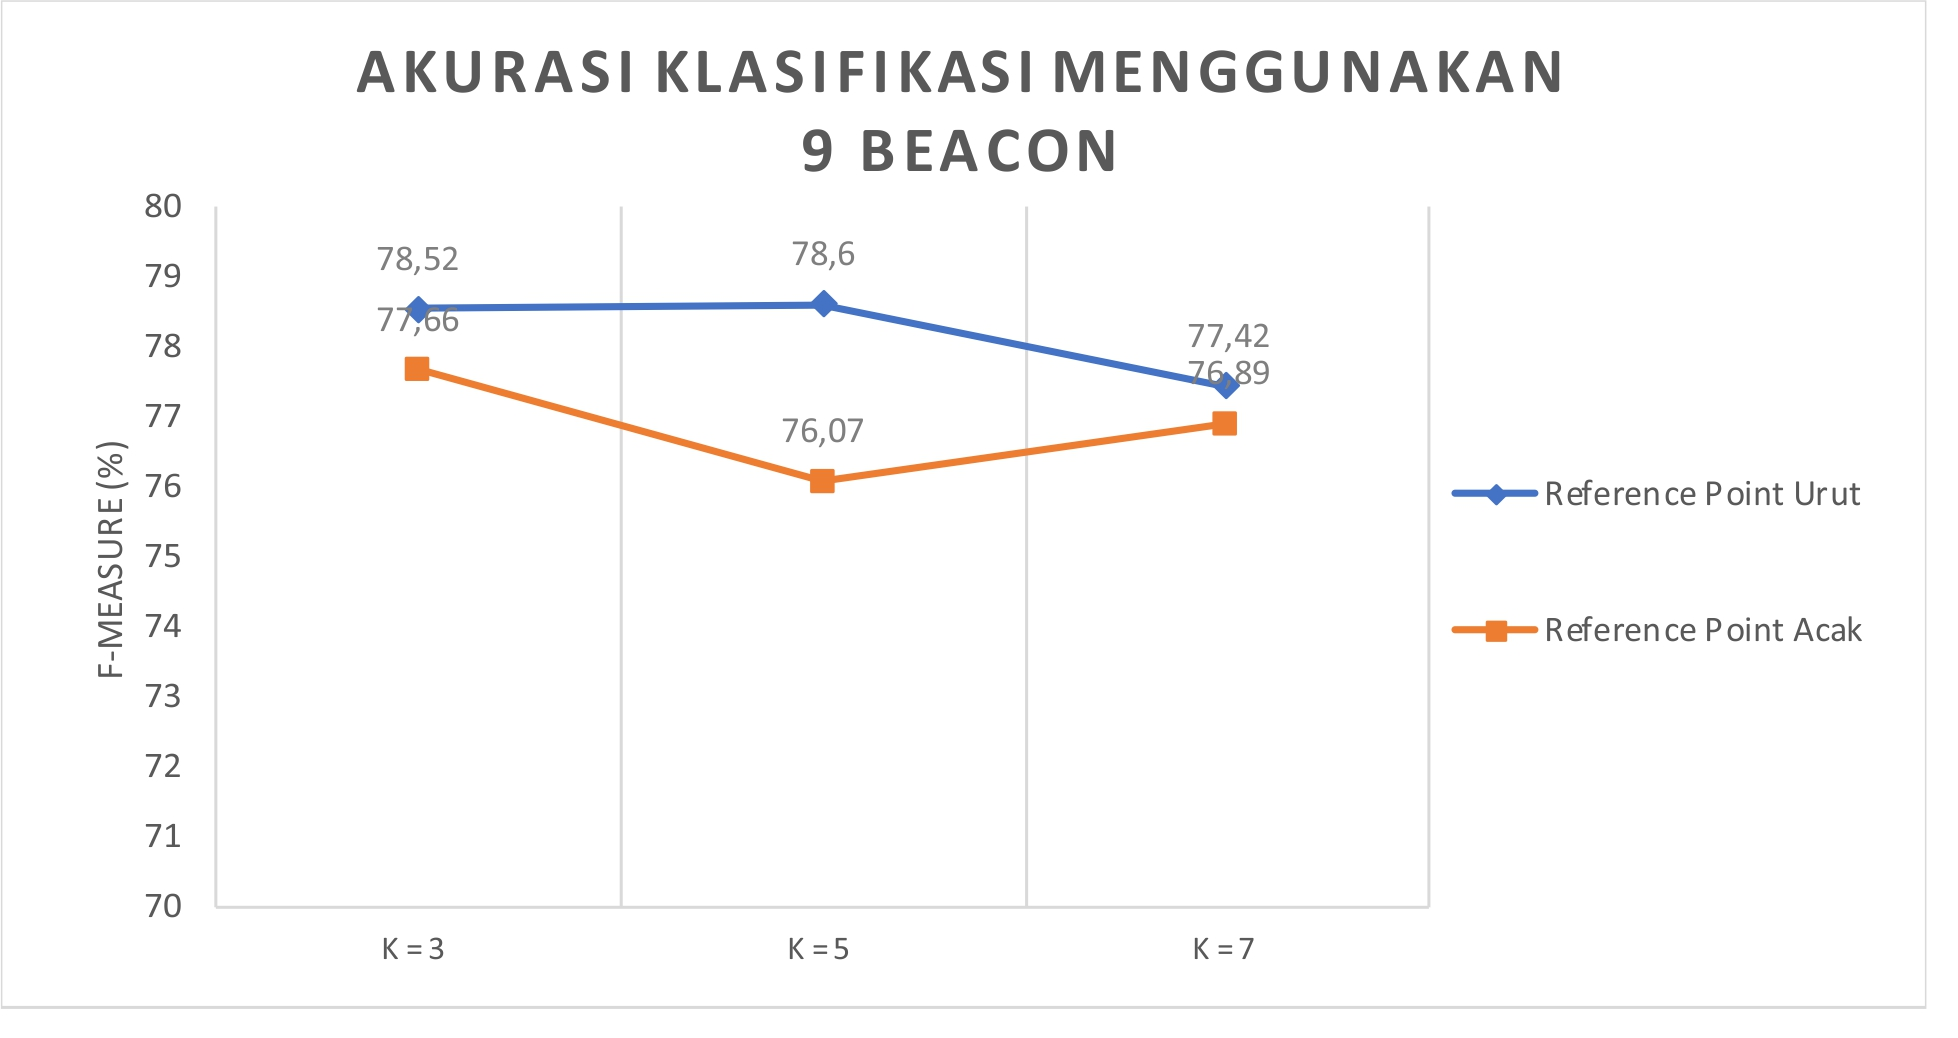
\includegraphics [width = 13cm, height= 7cm]{gambar/pengujian/grafik-akurasi-klasifikasi}}
		      \caption{Grafik Perbandingan F-Measure dengan Menggunakan Parameter Pengujian yang Berbeda.}
		      \label{gambar-grafik-akurasi-klasifikasi-9-beacon}
	      \end{figure}

	      \vspace{2cm}
	      \par Pengambilan data uji dilakukan untuk menguji tingkat keberhasilan klasifikasi dengan melihat akurasi tertinggi bergantung pada parameter nilai K yang digunakan. Pada pengujian ini terdapat titik yang sering salah diprediksi yaitu sebanyak 6 dari 6 kali pengujian. Lokasi titik yang sering salah diprediksi ditandai dengan lingkaran bewarna biru yang ditampilkan dalam bentuk ilustrasi denah yang dapat dilihat pada Gambar \ref{gambar-denah-titik-uji-b0302} dan Gambar \ref{gambar-denah-titik-uji-e0207}.
	      \vspace{0.2cm}
	      \begin{figure}[H]
		      \center
		      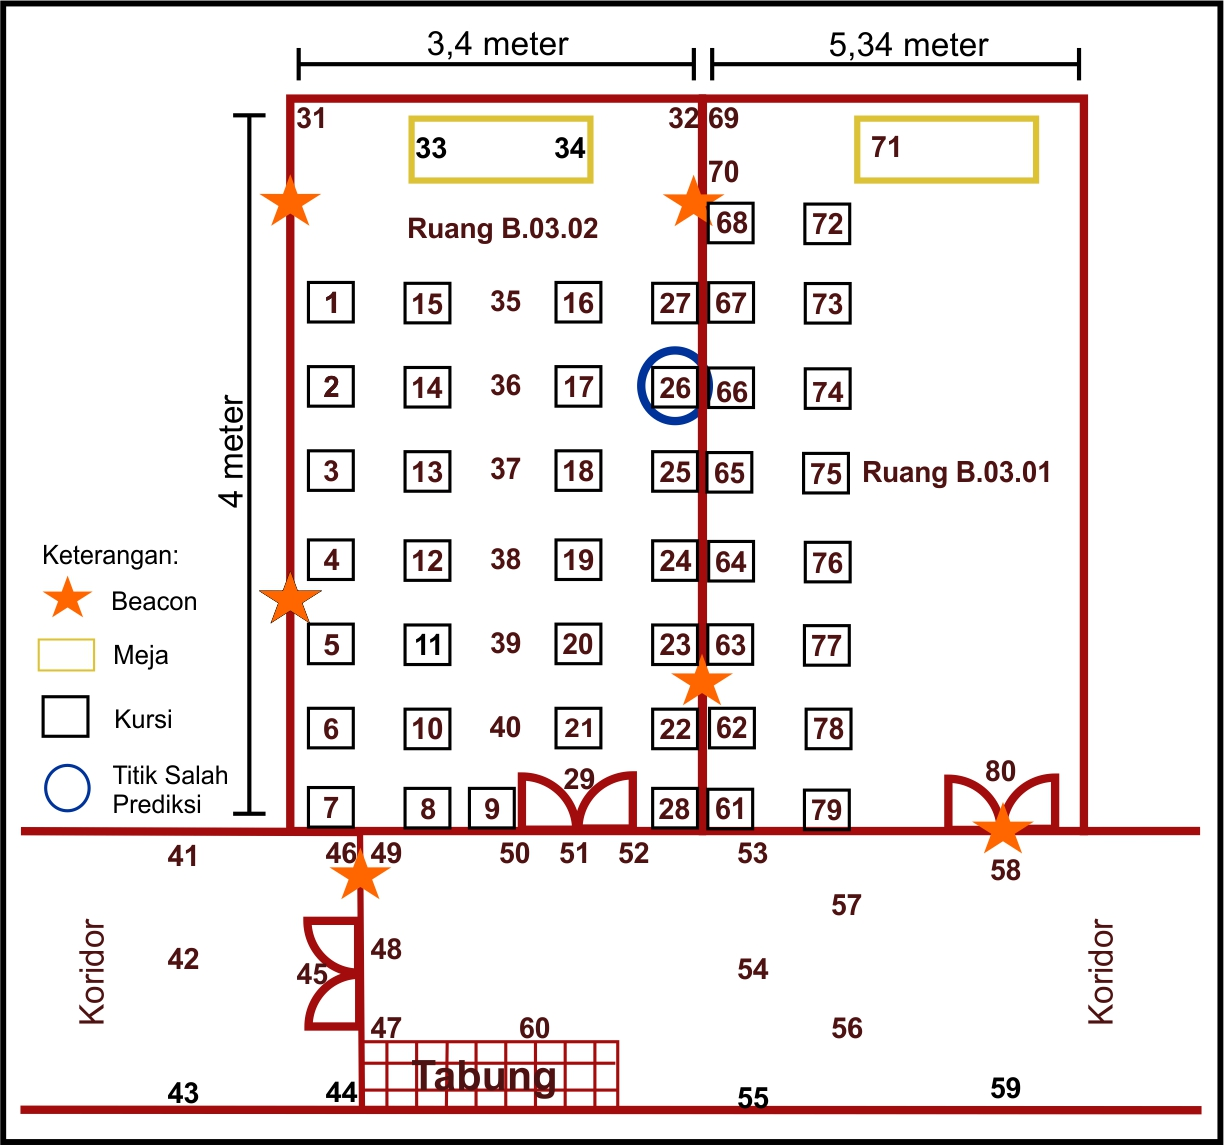
\includegraphics [width = 11cm, height= 9cm]{gambar/denah/B0302-Uji}
		      \caption{Lokasi Titik yang Sering Salah Diprediksi di Kelas B.03.02.}
		      \label{gambar-denah-titik-uji-b0302}
	      \end{figure}

	      \begin{figure}[H]
		      \center
		      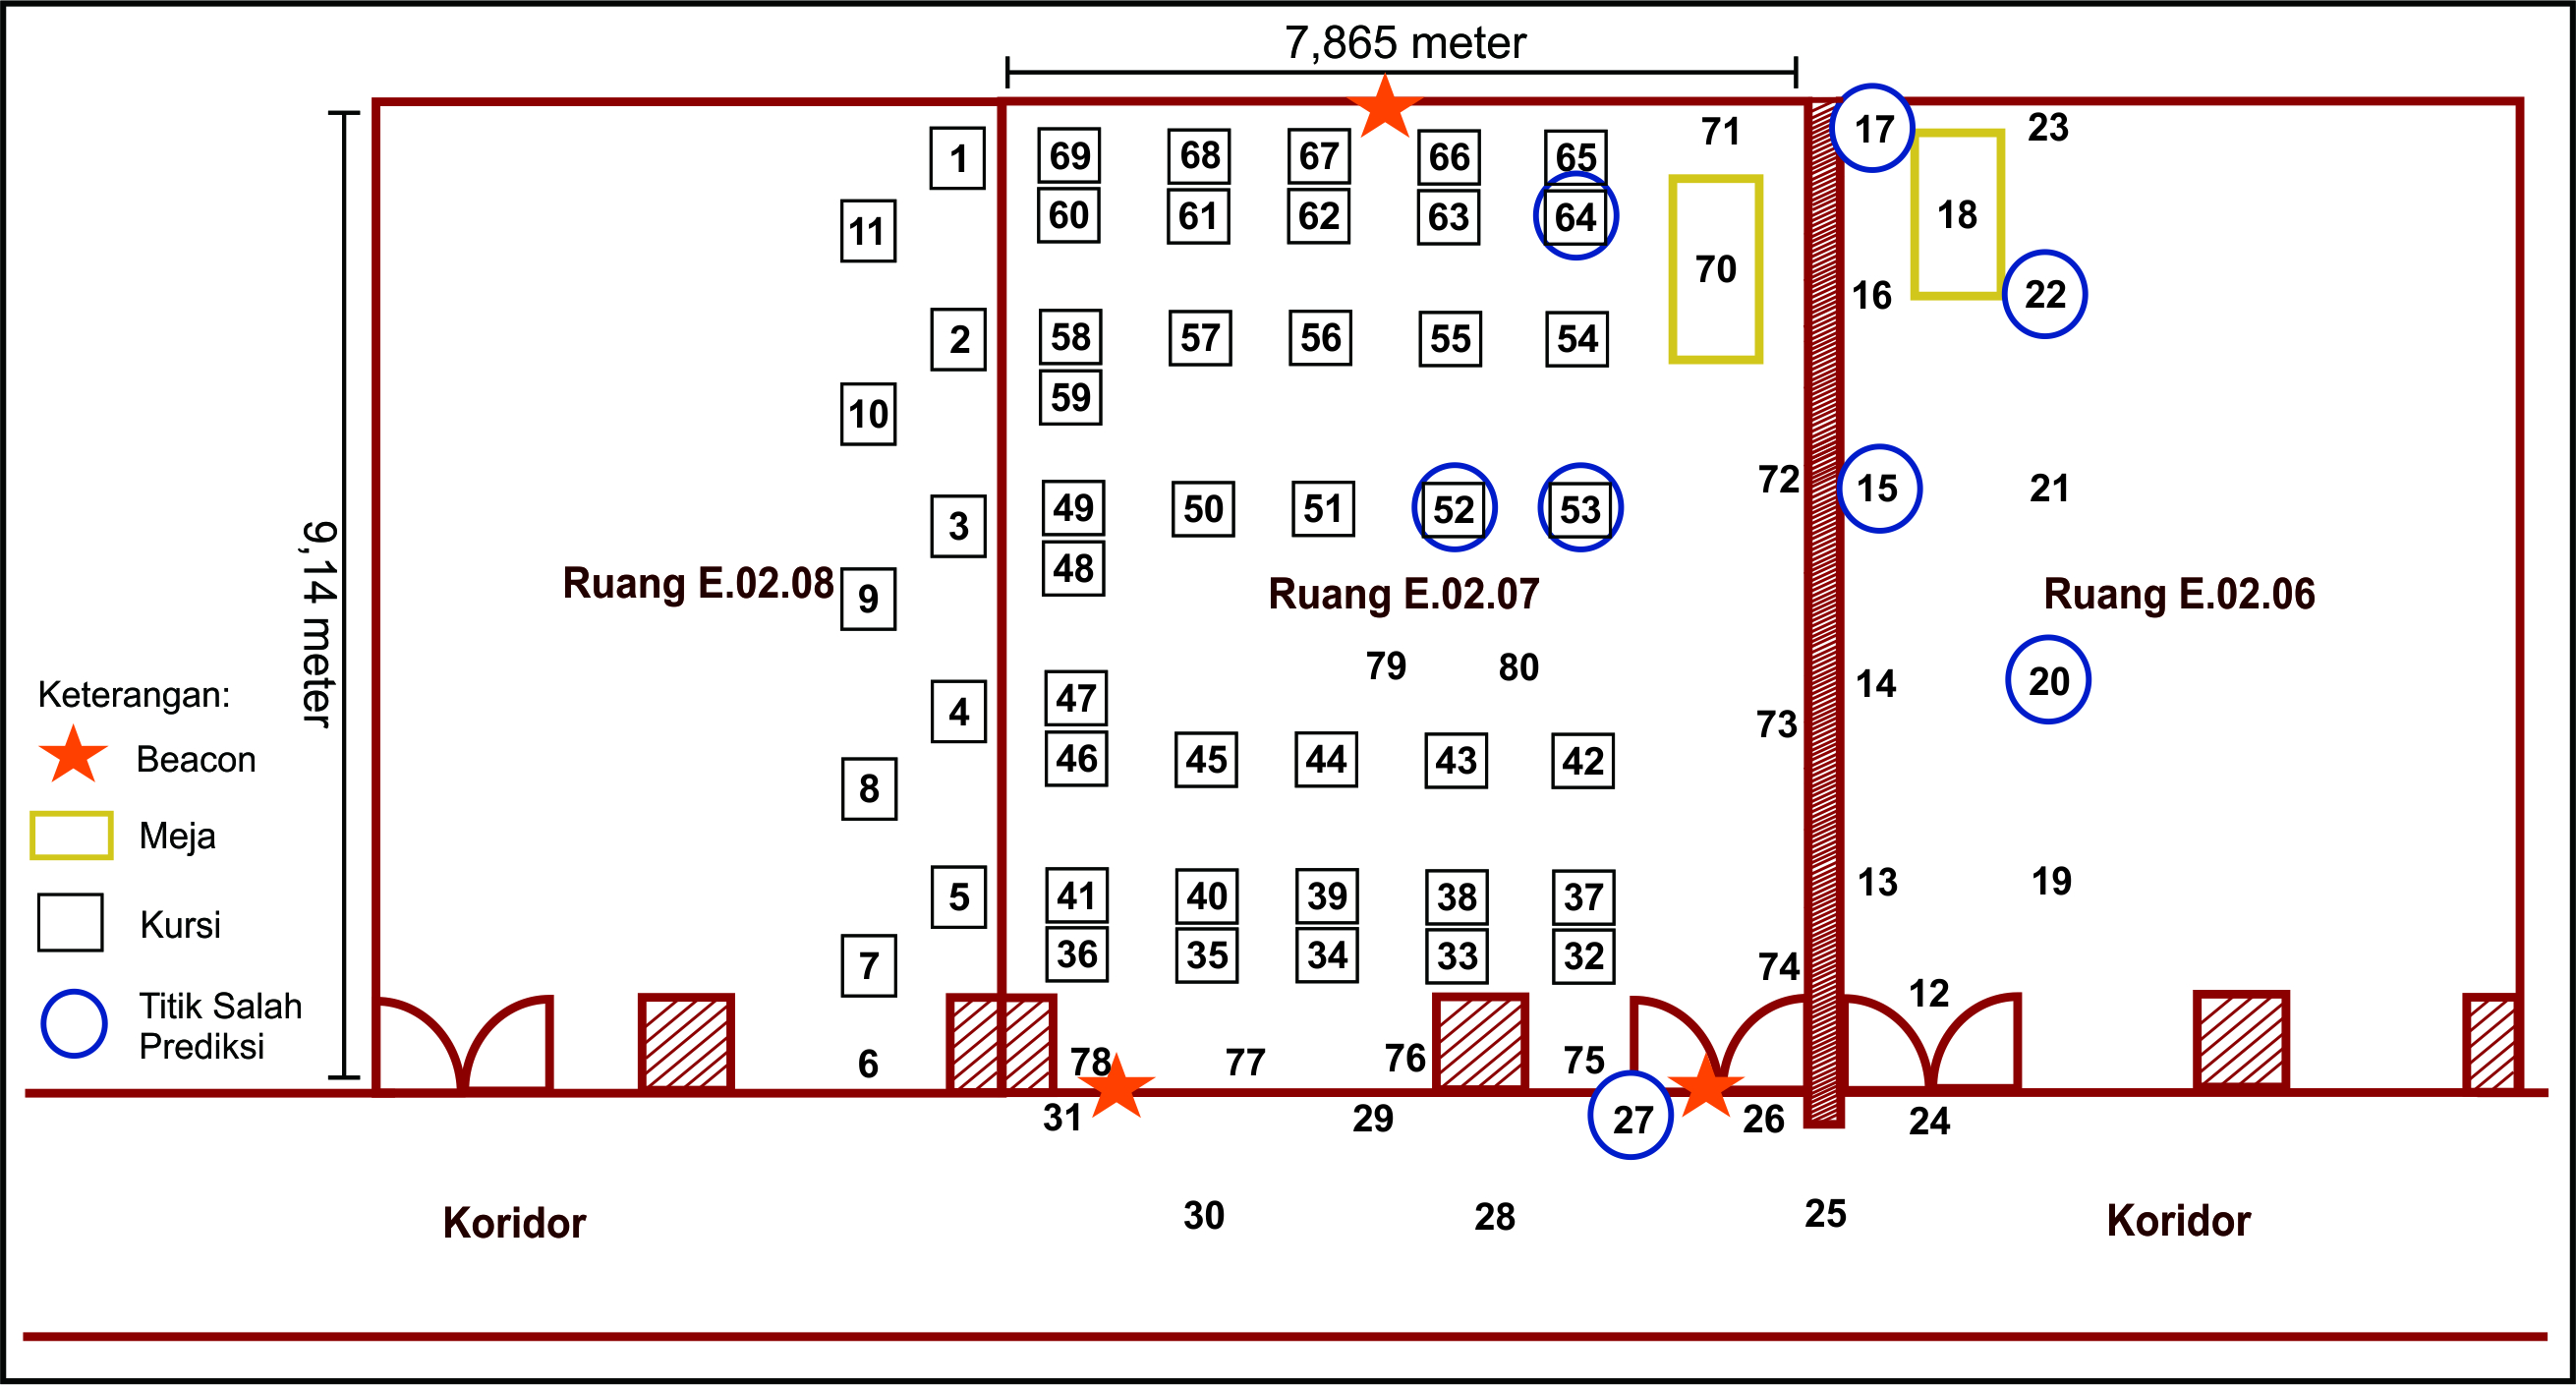
\includegraphics [width = 14cm, height= 8cm]{gambar/denah/E0207-Uji}
		      \caption{Lokasi Titik yang Sering Salah Diprediksi di Kelas E.02.07.}
		      \label{gambar-denah-titik-uji-e0207}
	      \end{figure}
	      %batas batas batas batas batas batas batas batas batas batas batas batas batas

	\item Pengujian Keakuratan Reference Point Berdasarkan Penggunaan Jumlah Beacon pada Ruang Kuliah B.03.02

	      \par Pengujian ini dianalisis menggunakan metode klasifikasi K-NN. Pengujian ini bertujuan untuk menganalisis tingkat keakuratan klasifikasi jenis \textit{reference point} terbaik yang digunakan dengan membandingkan penggunaan jumlah Beacon dengan melihat \textit{F-Measure} yang didapatkan dari setiap pengujian. Jumlah Beacon yang dibandingkan adalah 3 Beacon dan 6 Beacon. Data \textit{training} yang digunakan pada penelitian ini sebanyak 368 data kekuatan sinyal dengan masing-masing 120 data kekuatan sinyal untuk \textit{reference point} acak, 168 data kekuatan sinyal untuk \textit{reference point} urut dan 80 sebagai data uji. Pengumpulan data \textit{training} dilakukan dengan cara melakukan pemetaan kekuataan sinyal yang telah dijelaskan pada \textbf{BAB III}. Hasil dari proses pengujian metode klasifikasi K-NN menunjukkan bahwa dengan K=5 untuk data kekuatan sinyal \textit{reference point} acak menggunakan 6 Beacon, memiliki \textit{F-Measure} paling baik dengan nilai 96,20\% dibandingkan dengan parameter pengujian lainnya. Hasil pengujian menggunakan metode K-NN ini dapat dilihat secara detil pada Tabel \ref{tabelfmeasureee}.
	      Please add the following required packages to your document preamble:
	      %   \usepackage{multirow}
	      %   \begin{table}[H]
	      %       \fontsize{10}{12}\selectfont
	      %       \center
	      %       \caption{Perbandingan F-Measure}
	      %       \label{tabelfmeasureee}
	      %       \begin{tabular}{|c|c|l|c|c|c|}
	      % 	      \hline
	      % 	      Nilai K            & Jumlah BLE         & \multicolumn{1}{c|}{Jenis Titik} & Precision & Recall  & F-Measure \\ \hline
	      % 	      \multirow{2}{*}{3} & \multirow{2}{*}{3} & Urut                             & 67,24\%   & 97,50\% & 80,00\%   \\ \cline{3-6}
	      % 	                         &                    & Acak                             & 82,50\%   & 82,50\% & 82,50\%   \\ \hline
	      % 	      \multirow{2}{*}{5} & \multirow{2}{*}{3} & Urut                             & 67,24\%   & 97,50\% & 80,00\%   \\ \cline{3-6}
	      % 	                         &                    & Acak                             & 80,50\%   & 82,50\% & 81,50\%   \\ \hline
	      % 	      \multirow{2}{*}{7} & \multirow{2}{*}{3} & Urut                             & 67,24\%   & 97,50\% & 80,00\%   \\ \cline{3-6}
	      % 	                         &                    & Acak                             & 80,50\%   & 82,50\% & 81,50\%   \\ \hline
	      % 	      \multirow{2}{*}{3} & \multirow{2}{*}{6} & Urut                             & 90,70\%   & 97,50\% & 94,00\%   \\ \cline{3-6}
	      % 	                         &                    & Acak                             & 97,40\%   & 92,50\% & 95,00\%   \\ \hline
	      % 	      \multirow{2}{*}{5} & \multirow{2}{*}{6} & Urut                             & 90,70\%   & 97,50\% & 94,00\%   \\ \cline{3-6}
	      % 	                         &                    & Acak                             & 97,40\%   & 95,00\% & 96,20\%   \\ \hline
	      % 	      \multirow{2}{*}{7} & \multirow{2}{*}{6} & Urut                             & 90,70\%   & 97,50\% & 94,00\%   \\ \cline{3-6}
	      % 	                         &                    & Acak                             & 97,40\%   & 92,50\% & 95,00\%   \\ \hline
	      %       \end{tabular}
	      %   \end{table}

	      %   \par Ilustrasi dari perbandingan F-Measure setiap parameter pengujian ditampilkan pada Gambar \ref{gambar-grafik-akurasi-klasifikasi-6-beacon}.
	      %   \begin{figure}[H]
	      %       \center
	      %       \shadowbox
	      %       {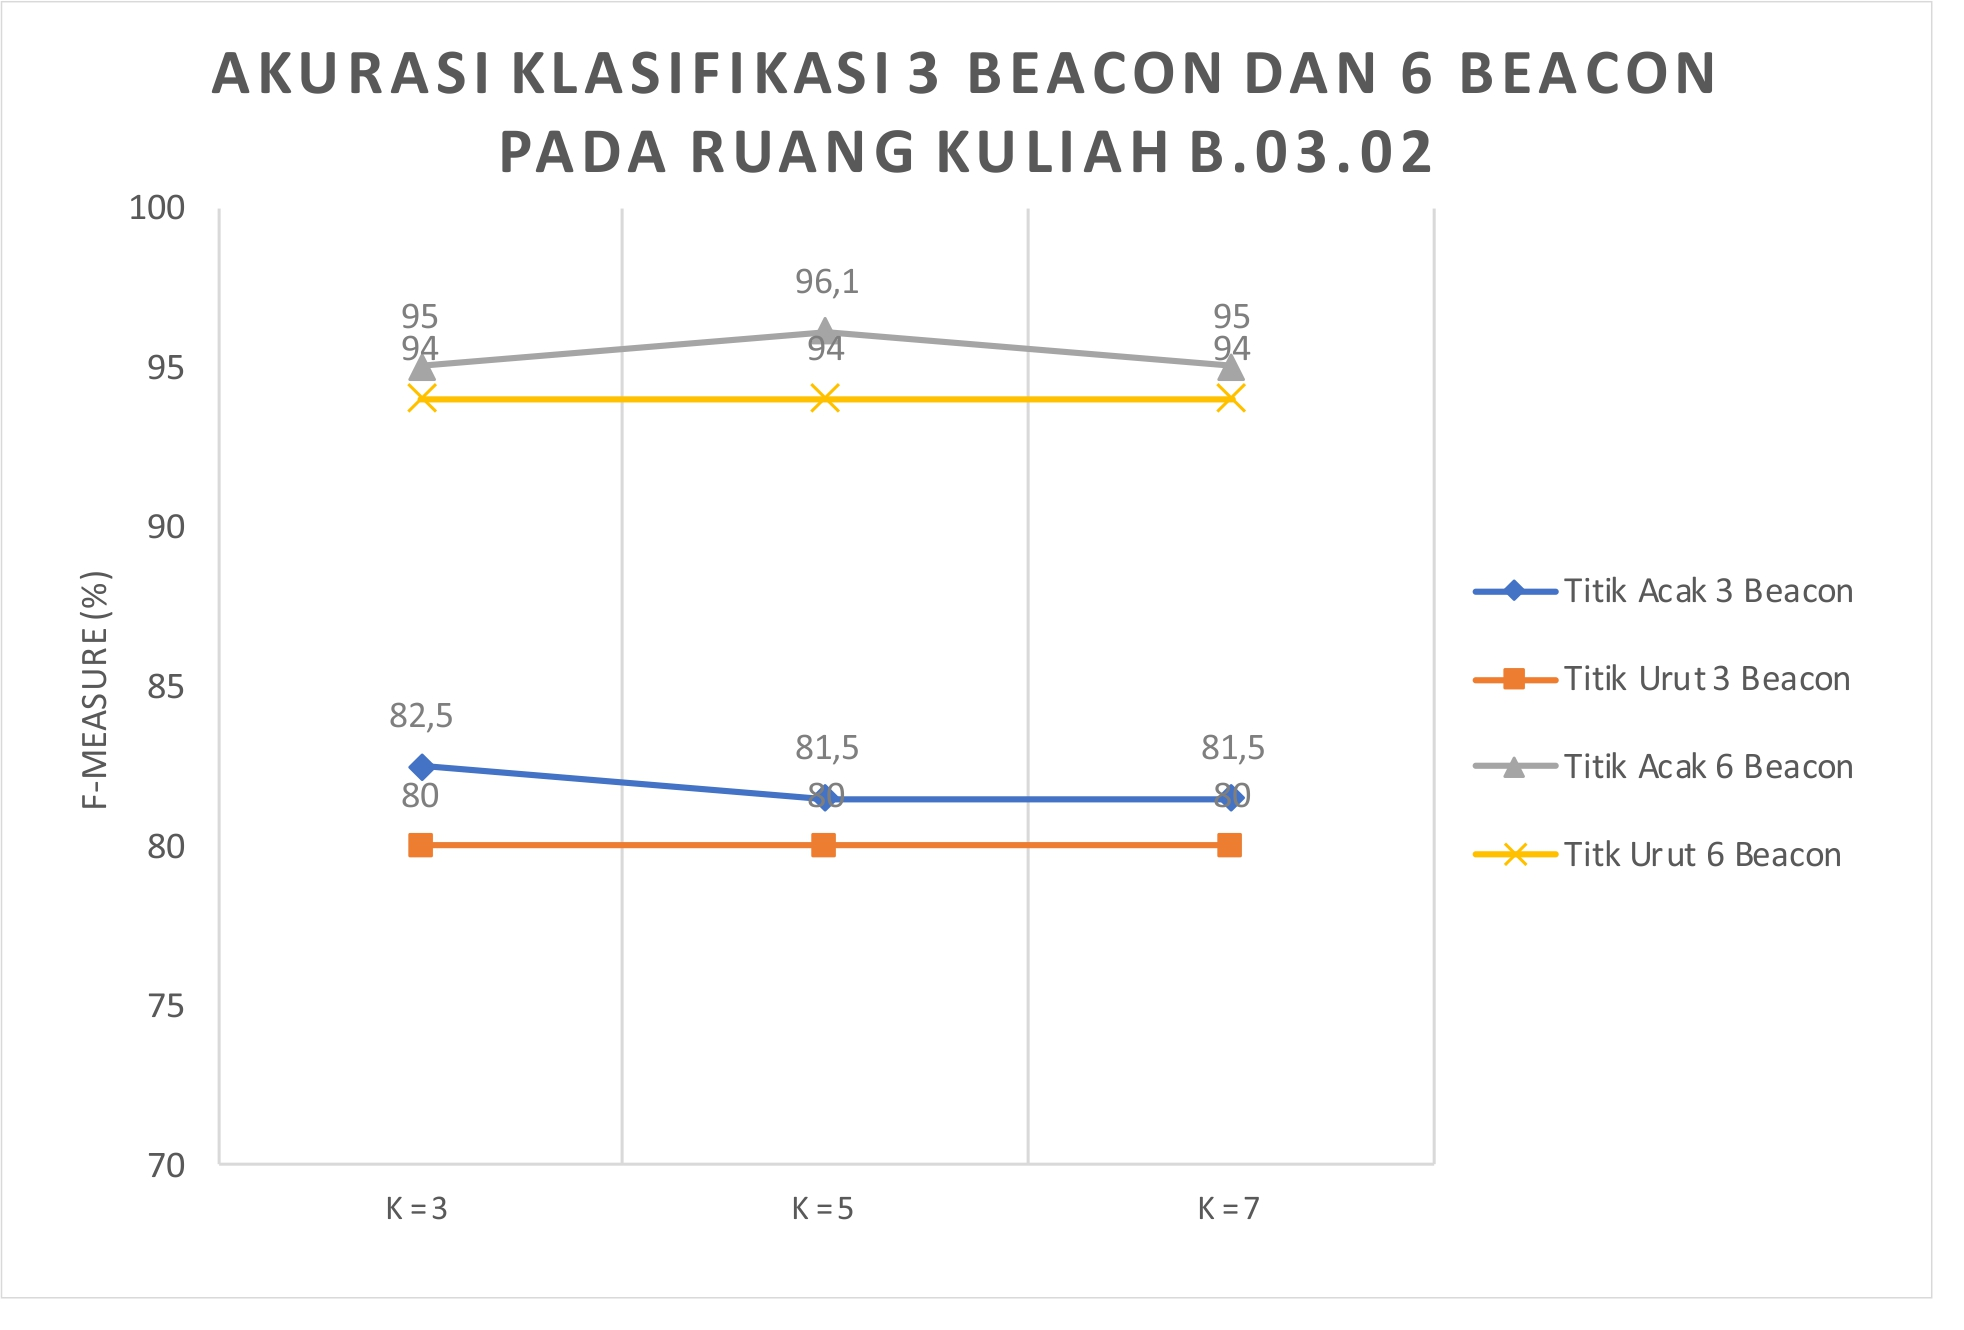
\includegraphics [width = 14cm, height= 8.7cm]{gambar/pengujian/grafik-akurasi-klasifikasi-kelas-b0302}}
	      %       \caption{Grafik Perbandingan F-Measure dengan Menggunakan Parameter Pengujian yang Berbeda.}
	      %       \label{gambar-grafik-akurasi-klasifikasi-6-beacon}
	      %   \end{figure}

	      %   \par Berdasarkan hasil pengujian dengan parameter nilai K yang berbeda menggunakan 3 Beacon dan 6 Beacon berdasarkan jenis \textit{reference point} yang digunakan, menunjukkan bahwa penggunaan 6 Beacon mengurangi kesalahan prediksi titik dibandingkan dengan 3 Beacon. Ilustrasi perbandingan tersebut dapat ditampilkan pada Gambar \ref{gambar-grafik-titik-salah-prediksi}.
	      %   \begin{figure}[H]
	      %       \center
	      %       \shadowbox
	      %       {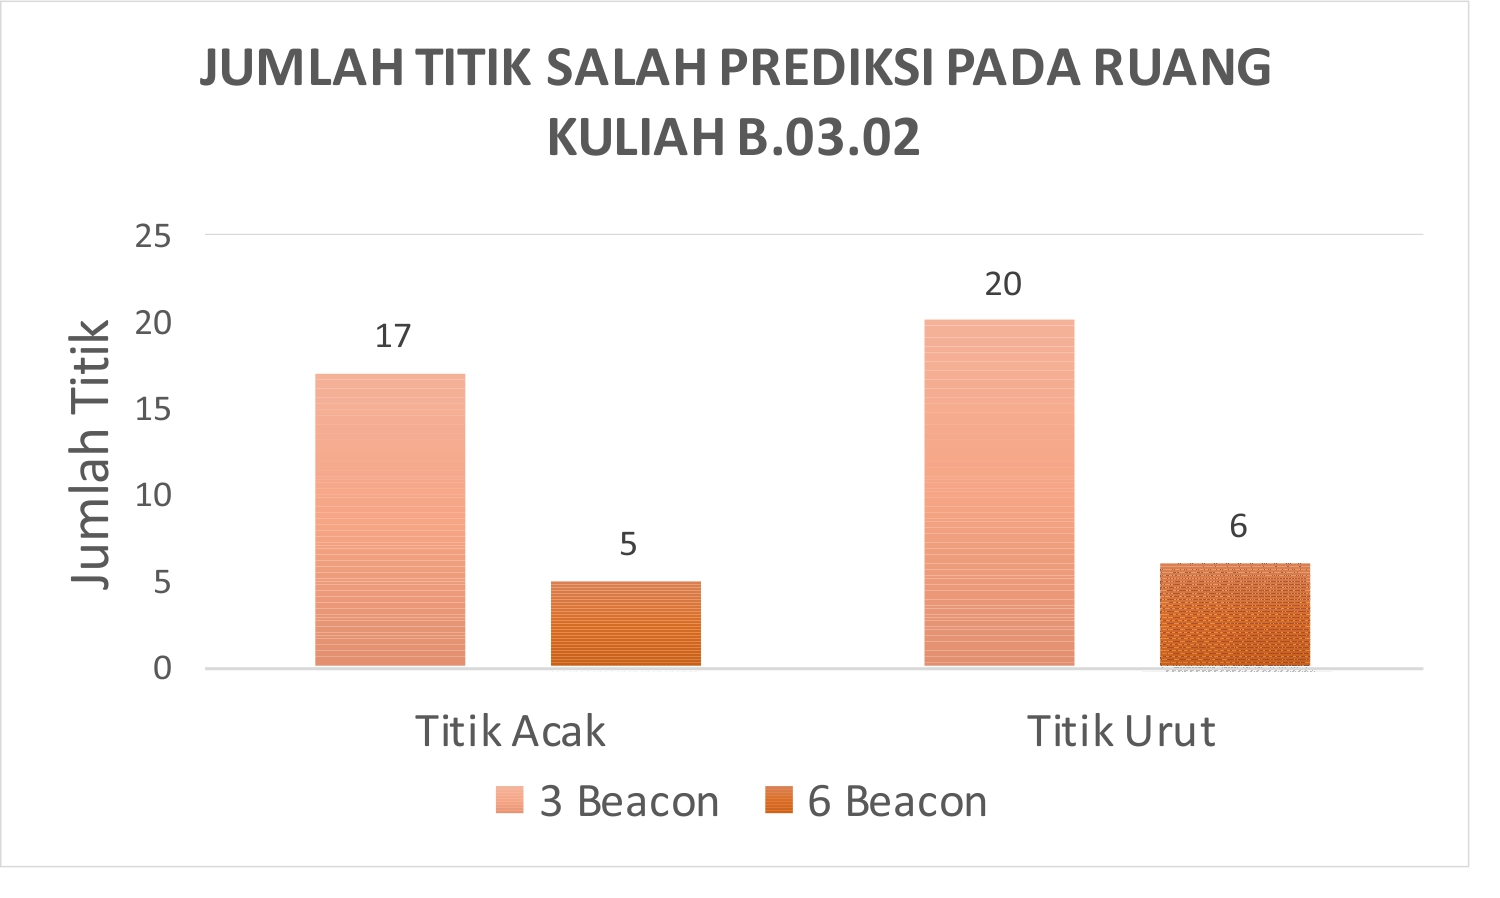
\includegraphics [width = 9cm, height= 5cm]{gambar/pengujian/grafik-titik-salah-prediksi}}
	      %       \caption{Grafik Jumlah Titik yang Salah Diprediksi.}
	      %       \label{gambar-grafik-titik-salah-prediksi}
	      %   \end{figure}


	      %batas batas batas batas batas batas batas batas batas batas batas batas batas	
\end{enumerate}

\subsection{Pengujian Usabilitas Menggunakan Metode UMUX}
\par Proses pengujian ini bertujuan untuk menguji kelayakan dan kegunaan dari sistem yang telah dibuat dan akan digunakan oleh pengguna. Sebelum melakukan pengujian ini, adapun \textit{Test Plan} yang telah dibuat untuk yang dapat dilihat pada Tabel \ref{testplan-aplikasi-utama}.

\begin{table}[H]
	\fontsize{10}{12}\selectfont
	\center
	\caption{\textit{Test Plan} Aplikasi SpecifyLocation}
	\label{testplan-aplikasi-utama}
	\begin{tabular}{|l|l|l|l|l|}
		\hline
		\multicolumn{5}{|c|}{\textbf{Test Plan Aplikasi SpecifyLocation}}                                                                                                                                                                                                                                                                                                                                                              \\ \hline
		\multicolumn{5}{|l|}{\begin{tabular}[c]{@{}l@{}}Lokasi:\\ Lantai 1 Gedung A FMIPA USK \\Lantai 3 Gedung A FMIPA USK\end{tabular}}                                                                                                                                                                                                                                                                                              \\ \hline
		\multicolumn{5}{|l|}{\begin{tabular}[c]{@{}l@{}}Skenario:\\ 1. Pengguna membuka aplikasi.\\ 2. Pengguna memahami tampilan halaman awal. \\ 3. Pengguna menekan cek lokasi di lantai 1 gedung a FMIPA USK. \\ 4. Pengguna menekan cek lokasi di lantai 3 gedung a FMIPA USK.\\ 5. Pengguna melihat hasil prediksi lokasi yang dilakukan oleh aplikasi.\\6. Pengguna melihat estimasi jumlah orang di dalam gedung\end{tabular}} \\ \hline
		\multicolumn{5}{|l|}{\begin{tabular}[c]{@{}l@{}}Alat:\\ 1. Smartphone Android\\ 2. Beacon\end{tabular}}                                                                                                                                                                                                                                                                                                                        \\ \hline
		\multicolumn{5}{|l|}{\begin{tabular}[c]{@{}l@{}}Hasil:\\ Hasil pengujian dapat dilihat pada tabel dan lampiran.\end{tabular}}                                                                                                                                                                                                                                                                                                  \\ \hline
	\end{tabular}
\end{table}

\par Pengujian UMUX dilakukan dengan memberikan kuisioner kepada responden. Isi kuisioner tersebut berisi 4 pertanyaan seperti yang sudah dibahas pada \textbf{BAB III}. Pengujian ini memiliki [Jumlah responden......] responden. Hasil skor pengujian metode UMUX yang dilakukan dapat dilihat pada tabel \ref{umux-aplikasi-utama} berikut.
% \par Pengujian dengan metode SUS dilakukan dengan memberikan kuisioner kepada responden. Kuisioner tersebut berisi 10 pertanyaan seperti yang telah dibahas pada. Pengujian Aplikasi Kehadiran Dosen memiliki responden berjumlah 5 orang sedangkan pengujian Aplikasi Kehadiran Mahasiswa memiliki responden berjumlah 9 orang. Hasil skor pengujian metode SUS yang dilakukan dapat dilihat pada Tabel \ref{sus-aplikasi-dosen} dan Tabel \ref{sus-aplikasi-mahasiswa} berikut.
%TABEL SUS APLIKASI DOSEN%
\begin{table}[H]
	\centering
	\caption{\textit{Usability Testing} dengan menggunakan metode UMUX}
	\label{UMUX}
	\begin{tabular}{|ccccc|c|}
		\hline
		\rowcolor[HTML]{EFEFEF}
		\multicolumn{1}{|c|}{\cellcolor[HTML]{EFEFEF}}                            & \multicolumn{4}{c|}{\cellcolor[HTML]{EFEFEF}Kode Pertanyaan} & \cellcolor[HTML]{EFEFEF}                                                                                                                                     \\ \cline{2-5}
		\rowcolor[HTML]{EFEFEF}
		\multicolumn{1}{|c|}{\multirow{-2}{*}{\cellcolor[HTML]{EFEFEF}Responden}} & \multicolumn{1}{c|}{\cellcolor[HTML]{EFEFEF}P1}              & \multicolumn{1}{c|}{\cellcolor[HTML]{EFEFEF}P2} & \multicolumn{1}{c|}{\cellcolor[HTML]{EFEFEF}P3} & P4 & \multirow{-2}{*}{\cellcolor[HTML]{EFEFEF}Skor UMUX} \\ \hline
		\multicolumn{1}{|c|}{1}                                                   & \multicolumn{1}{c|}{}                                        & \multicolumn{1}{c|}{}                           & \multicolumn{1}{c|}{}                           &    &                                                     \\ \hline
		\multicolumn{1}{|c|}{2}                                                   & \multicolumn{1}{c|}{}                                        & \multicolumn{1}{c|}{}                           & \multicolumn{1}{c|}{}                           &    &                                                     \\ \hline
		\multicolumn{1}{|c|}{3}                                                   & \multicolumn{1}{c|}{}                                        & \multicolumn{1}{c|}{}                           & \multicolumn{1}{c|}{}                           &    &                                                     \\ \hline
		\multicolumn{1}{|c|}{4}                                                   & \multicolumn{1}{c|}{}                                        & \multicolumn{1}{c|}{}                           & \multicolumn{1}{c|}{}                           &    &                                                     \\ \hline
		\multicolumn{1}{|c|}{5}                                                   & \multicolumn{1}{c|}{}                                        & \multicolumn{1}{c|}{}                           & \multicolumn{1}{c|}{}                           &    &                                                     \\ \hline
		\multicolumn{1}{|c|}{6}                                                   & \multicolumn{1}{c|}{}                                        & \multicolumn{1}{c|}{}                           & \multicolumn{1}{c|}{}                           &    &                                                     \\ \hline
		\multicolumn{1}{|c|}{7}                                                   & \multicolumn{1}{c|}{}                                        & \multicolumn{1}{c|}{}                           & \multicolumn{1}{c|}{}                           &    &                                                     \\ \hline
		\multicolumn{1}{|c|}{8}                                                   & \multicolumn{1}{c|}{}                                        & \multicolumn{1}{c|}{}                           & \multicolumn{1}{c|}{}                           &    &                                                     \\ \hline
		\multicolumn{1}{|c|}{9}                                                   & \multicolumn{1}{c|}{}                                        & \multicolumn{1}{c|}{}                           & \multicolumn{1}{c|}{}                           &    &                                                     \\ \hline
		\multicolumn{1}{|c|}{10}                                                  & \multicolumn{1}{c|}{}                                        & \multicolumn{1}{c|}{}                           & \multicolumn{1}{c|}{}                           &    &                                                     \\ \hline
		\multicolumn{1}{|c|}{11}                                                  & \multicolumn{1}{c|}{}                                        & \multicolumn{1}{c|}{}                           & \multicolumn{1}{c|}{}                           &    &                                                     \\ \hline
		\multicolumn{1}{|c|}{12}                                                  & \multicolumn{1}{c|}{}                                        & \multicolumn{1}{c|}{}                           & \multicolumn{1}{c|}{}                           &    &                                                     \\ \hline
		\multicolumn{1}{|c|}{13}                                                  & \multicolumn{1}{c|}{}                                        & \multicolumn{1}{c|}{}                           & \multicolumn{1}{c|}{}                           &    &                                                     \\ \hline
		\multicolumn{1}{|c|}{14}                                                  & \multicolumn{1}{c|}{}                                        & \multicolumn{1}{c|}{}                           & \multicolumn{1}{c|}{}                           &    &                                                     \\ \hline
		\multicolumn{1}{|c|}{15}                                                  & \multicolumn{1}{c|}{}                                        & \multicolumn{1}{c|}{}                           & \multicolumn{1}{c|}{}                           &    &                                                     \\ \hline
		\multicolumn{1}{|c|}{16}                                                  & \multicolumn{1}{c|}{}                                        & \multicolumn{1}{c|}{}                           & \multicolumn{1}{c|}{}                           &    &                                                     \\ \hline
		\multicolumn{1}{|c|}{17}                                                  & \multicolumn{1}{c|}{}                                        & \multicolumn{1}{c|}{}                           & \multicolumn{1}{c|}{}                           &    &                                                     \\ \hline
		\multicolumn{1}{|c|}{18}                                                  & \multicolumn{1}{c|}{}                                        & \multicolumn{1}{c|}{}                           & \multicolumn{1}{c|}{}                           &    &                                                     \\ \hline
		\multicolumn{1}{|c|}{19}                                                  & \multicolumn{1}{c|}{}                                        & \multicolumn{1}{c|}{}                           & \multicolumn{1}{c|}{}                           &    &                                                     \\ \hline
		\multicolumn{1}{|c|}{20}                                                  & \multicolumn{1}{c|}{}                                        & \multicolumn{1}{c|}{}                           & \multicolumn{1}{c|}{}                           &    &                                                     \\ \hline
		\rowcolor[HTML]{EFEFEF}
		\multicolumn{5}{|c|}{\cellcolor[HTML]{EFEFEF}Rata - Rata}                 &                                                                                                                                                                                                                             \\ \hline
	\end{tabular}
\end{table}

\par Berdasarkan hasil pengujian usabilitas menggunakan metode UMUX yang telah dilakukan diatas, hasil rata-rata pengujian Aplikasi LocaLization mendapatkan skor sebesar ....\% . Berdasarkan skor tersebut, maka aplikasi LocaLization ini memiliki skor interpretasi \textbf{"dapat diterima"} berdasarkan Tabel 3.4.

\subsection{Pengujian Fungsionalitas Menggunakan Blackbox}
\par Tujuan pengujian \textit{blackbox} adalah untuk menguji fungsionalitas dari aplikasi yang telah dibuat dengan cara menjalankan aplikasi tersebut apakah sesuai dengan alur bisnis yang diinginkan atau tidak. Proses ini melihat fungsi yang tidak sesuai pada aplikasi dan kesalahan-kesalahan aplikasi dalam mengerjakan suatu perintah. Pengujian \textit{blackbox} dilakukan pada aplikasi utama berbasis android yaitu aplikasi LocaLization dan aplikasi \textit{web monitoring}. Beberapa fitur aplikasi yang diuji menggunakan metode \textit{blackbox} dapat dilihat pada Tabel \ref{blackbox-aplikasi-utama}, dan Tabel \ref{blackbox-web-monitoring}

%BLACKBOX APLIKASI LocaLization%

\begin{table}[H]
	\center
	\caption{Pengujian \textit{Blackbox} Aplikasi LocaLization}
	\label{blackbox-aplikasi-utama}
	\begin{tabular}{|c|l|l|l|c|}
		\hline
		\textbf{No} & \multicolumn{1}{c|}{\textbf{Nama Pengujian}}                                      & \multicolumn{1}{c|}{\textbf{Skenario}}                                                                             & \multicolumn{1}{c|}{\textbf{Tampilan}}                                                                           & \textbf{Hasil} \\ \hline
		1           & \begin{tabular}[c]{@{}l@{}}Menghidupkan\\ Bluetooth\end{tabular}                  & \begin{tabular}[c]{@{}l@{}}Tekan tombol\\ "Allow" pada\\ notifikasi yang\\ muncul\end{tabular}                     & \begin{tabular}[c]{@{}l@{}}Bluetooth akan\\ hidup\end{tabular}                                                   & Berhasil       \\ \hline
		2           & \begin{tabular}[c]{@{}l@{}}Lakukan proses\\ pemindaian \\ sinyal BLE\end{tabular} & \begin{tabular}[c]{@{}l@{}}Tekan tombol\\ "Cek Lokasi"\\ saat berada di dalam \\ gedung A\\ FMIPA USK\end{tabular} & \begin{tabular}[c]{@{}l@{}}Diarahkan ke\\ halaman denah\\ gedung A\\ FMIPA USK\end{tabular}                      & Berhasil       \\ \hline
		3           & \begin{tabular}[c]{@{}l@{}}Lakukan proses\\ pemindaian\\ sinyal BLE\end{tabular}  & \begin{tabular}[c]{@{}l@{}}Tekan tombol\\ "Cek Lokasi"\\ saat berada di luar gedung\\ A FMIPA USK\end{tabular}     & \begin{tabular}[c]{@{}l@{}}Diarahkan ke\\ halaman luar\\ gedung\end{tabular}                                     & Berhasil       \\ \hline
		4           & \begin{tabular}[c]{@{}l@{}}Melihat denah\\ dengan keterangan\\ warna\end{tabular} & Menggeser gambar Denah                                                                                             & \begin{tabular}[c]{@{}l@{}}Gambar denah\\ berwarna sesuai\\ dengan keterangannya\end{tabular}                    & Berhasil       \\ \hline
		5           & \begin{tabular}[c]{@{}l@{}}Melihat detail\\ Jumlah orang\end{tabular}             & \begin{tabular}[c]{@{}l@{}}Tekan tombol\\ "Jumlah Orang"\end{tabular}                                              & \begin{tabular}[c]{@{}l@{}}Diarahkan ke halaman\\ detail jumlah orang di\\ setiap posisi di gedung \end{tabular} & Berhasil       \\ \hline
	\end{tabular}
\end{table}

% BLACKBOX WEB Monitoring%
\begin{table}[H]
	\centering
	\caption{Pengujian \textit{Blackbox} Aplikasin Web Monitoring}
	\label{blackbox-web-monitoring}
	\begin{tabular}{|c|l|l|l|c|}
		\hline
		\textbf{No} & \multicolumn{1}{c|}{\textbf{Nama Pengujian}}                                & \multicolumn{1}{c|}{\textbf{Skenario}}                                                                                               & \multicolumn{1}{c|}{\textbf{Tampilan}}                                                                                                   & \textbf{Hasil} \\ \hline
		1           & \begin{tabular}[c]{@{}l@{}}Melihat halaman\\ \textit{Dashbord}\end{tabular} & \begin{tabular}[c]{@{}l@{}}Masuk ke halaman\\ \textit{web monitoring}\\ https://web-monitoring-\\ five.vercel.app/admin\end{tabular} & \begin{tabular}[c]{@{}l@{}}Muncul Halaman\\ dashbord serta total\\ pengguna yang\\ menggunakan\\ algoritma KMeans\\ dan SVM\end{tabular} & Berhasil       \\ \hline
		2           & \begin{tabular}[c]{@{}l@{}}Melihat detail\\ algoritma SVM\end{tabular}      & \begin{tabular}[c]{@{}l@{}}Tekan pilihan\\ "Algoritma SVM"\end{tabular}                                                              & \begin{tabular}[c]{@{}l@{}}Muncul detail estimasi\\ pengguna algoritma\\ SVM serta\\ keterangannya\end{tabular}                          & Berhasil       \\ \hline
		3           & \begin{tabular}[c]{@{}l@{}}Melihat detail\\ algoritma K-Means\end{tabular}  & \begin{tabular}[c]{@{}l@{}}Tekan pilihan\\ "Algoritma K-Means"\end{tabular}                                                          & \begin{tabular}[c]{@{}l@{}}Muncul detail estimasi\\ pengguna algoritma\\ K-Means serta\\ keterangannya\end{tabular}                      & Berhasil       \\ \hline
	\end{tabular}
\end{table}

%AKHIR DARI TABEL%
\par Berdasarkan hasil \textit{Blackbox Testing} dari tabel diatas menunjukkan bahwa Aplikasi utama berbasis android yaitu Aplikasi LocaLization dan Aplikasi Web Monitoring dapat berjalan dengan baik dibuktikan dengan  \textbf{"berhasil"} pada kolom hasil pengujian masing-masing fitur yang dikerjakan.


\begin{comment}
\bibliography{daftar-pustaka}
\end{comment}